\documentclass[a4paper,12pt,landscape]{mwart}
\usepackage[utf8]{inputenc}
\usepackage[T1]{fontenc}
\usepackage[MeX,plmath]{polski} 
\usepackage[usenames,dvipsnames]{xcolor}
\usepackage{tikz}
\usepackage{epsfig}
\usepackage{amsmath}
\usepackage{amssymb, xcolor}
\usepackage{multicol, url}
\usepackage{vwcol}
\usepackage{fancyhdr}
\usetikzlibrary{arrows.meta}
\usetikzlibrary{shapes.geometric}
\usepackage[unicode]{hyperref}
\usepackage{geometry}
\usepackage{fancypar}
\usepackage{anyfontsize}
\usepackage{blindtext}
\usepackage{multicol}
\usepackage{hyperref}
\usetikzlibrary{matrix}
\usepackage{ccfonts}
\newgeometry{tmargin=0.5cm, bmargin=0.5cm, lmargin=0.8cm, rmargin=0.8cm}
\begin{document}
\pagestyle{empty}
\pagecolor{Dandelion!20}
\title{\Huge{MAPA POLITECHNIKI ŚLĄSKIEJ}}
\author{Sandra Świeczak}
\maketitle
\begin{center}



\begin{tikzpicture}[scale=1.8]

\draw[very thick]
\foreach \i in {1,2,...,12} {%
  [rotate=(\i-1)*30] 
 (0:2)  arc (0:15:2) {[rounded corners=2pt] -- ++(15: 0.3)  arc (15:30:2.3) } -- ++(30: -0.3) 
};
\filldraw[SkyBlue!40] (0,0) circle (40pt);
\filldraw[YellowGreen,very thick] (-1.4,0) to[out=30,in=-190](0,0.5)to[out=-10,in=-170] (1.4,0);

\begin{scope}
    \clip (1.4,0) rectangle (-1.4,-1.4);
    \filldraw [YellowGreen](0,0) circle(1.4);
\end{scope}
\end{tikzpicture}
\end{center}
\newpage
\begin{center}

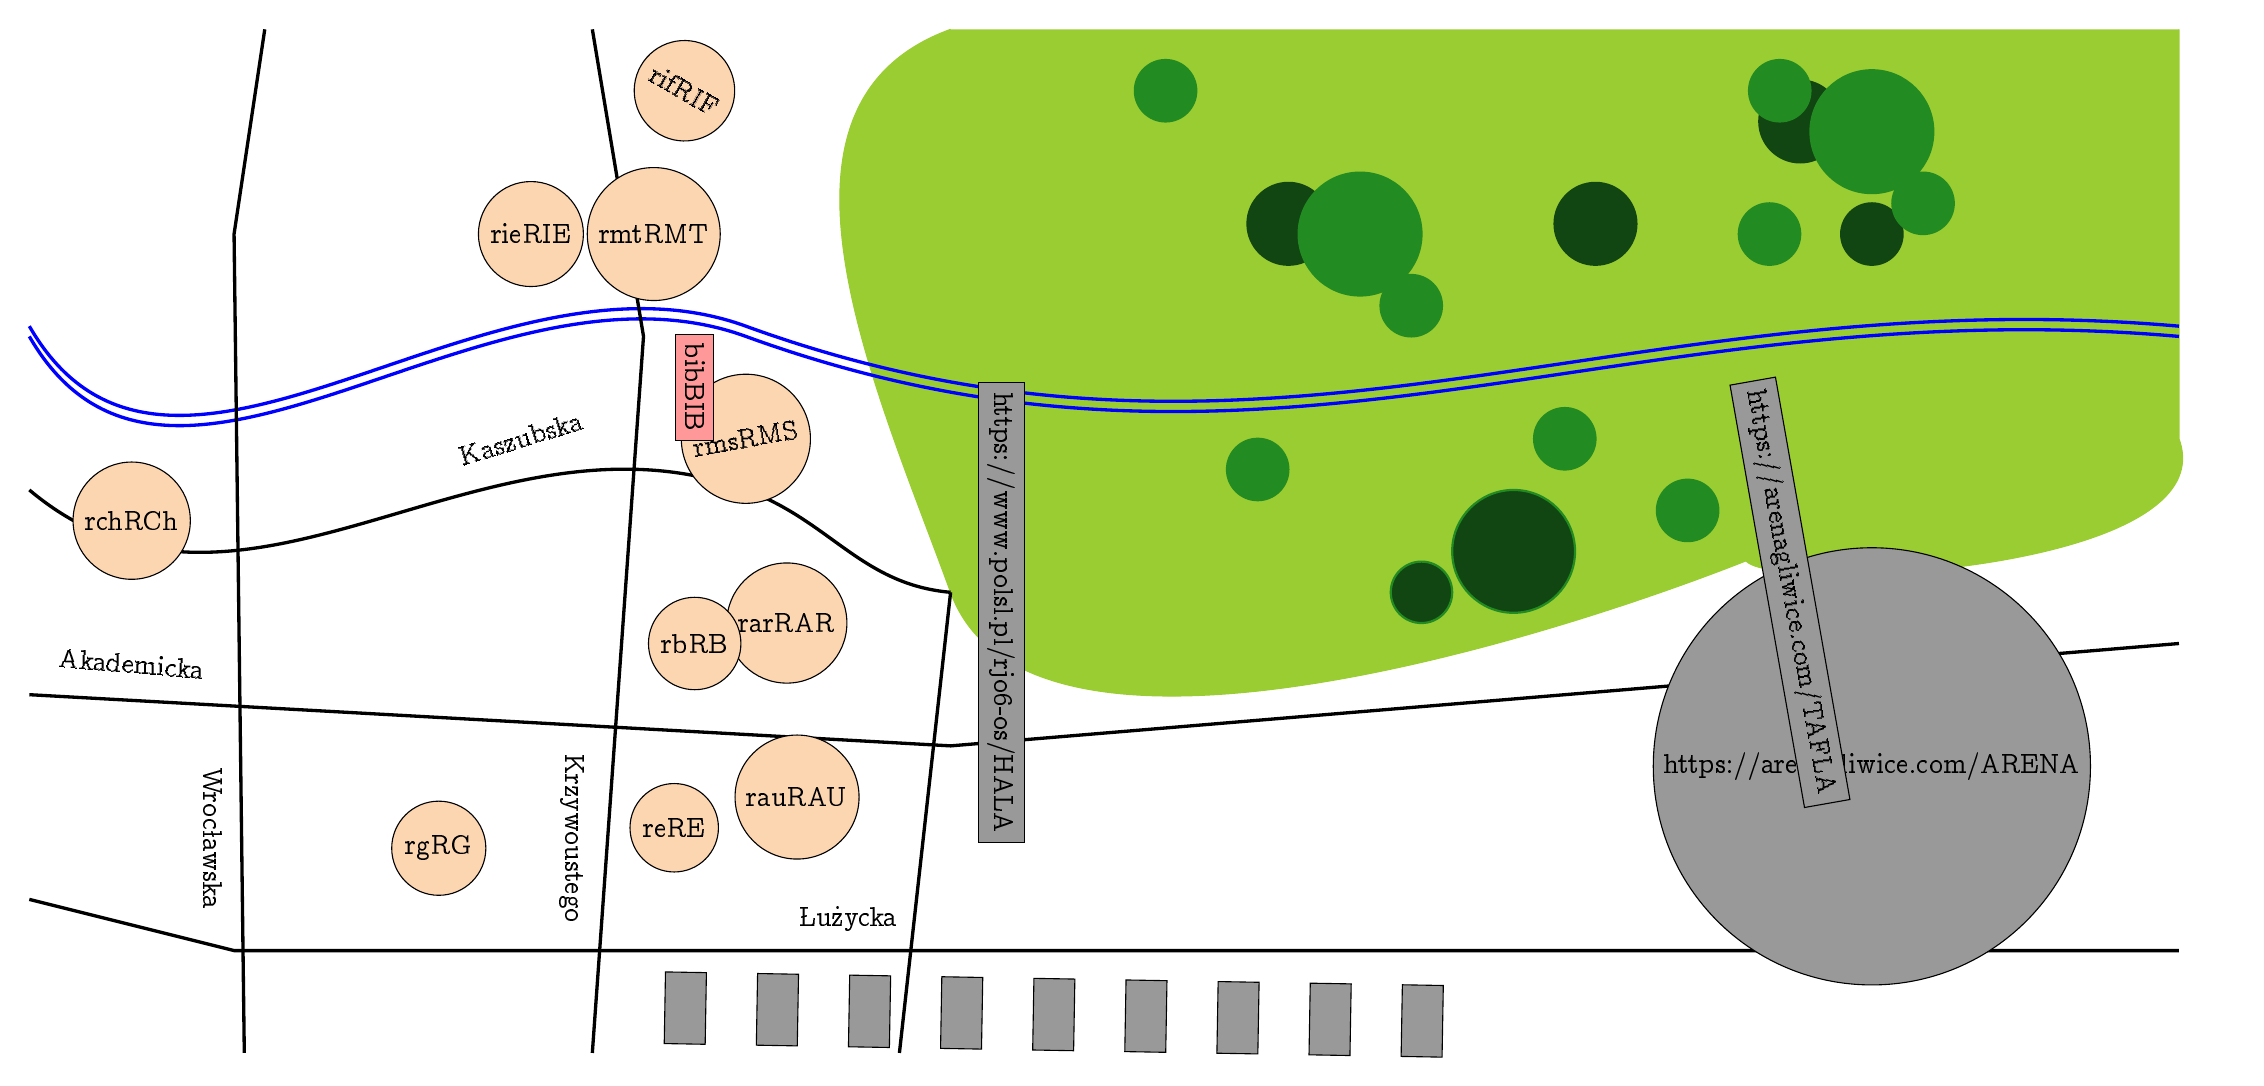
\begin{tikzpicture}[scale=1.3,fill=Apricot!50]

%%%%%%%%%%%%%%%%%%%%%%%%%%%% tereny zielone %%%%%%%%%%%%%%%%%%%%%%%%%%%%%%%%%%%% 

\draw[fill,YellowGreen](21,10) to (21,6) to[out=-70,in=-160](17,5)to [out=20, in=-70](9,4.5) to [out=110, in=-160](9,10);

\draw[color=ForestGreen!50!black, fill=ForestGreen!50!black, thick] (18,8) circle (0.3);
\draw[color=ForestGreen!50!black, fill=ForestGreen!50!black, thick] (17.3,9.1) circle (0.4);
\draw[color=ForestGreen, fill=ForestGreen, thick] (17,8) circle (0.3);
\draw[color=ForestGreen, fill=ForestGreen, thick] (18,9) circle (0.6);
\draw[color=ForestGreen, fill=ForestGreen, thick] (18.5,8.3) circle (0.3);
\draw[color=ForestGreen, fill=ForestGreen, thick] (17.1,9.4) circle (0.3);
\draw[color=ForestGreen!50!black, fill=ForestGreen!50!black, thick] (12.3,8.1) circle (0.4);
\draw[color=ForestGreen, fill=ForestGreen, thick] (12,5.7) circle (0.3);
\draw[color=ForestGreen, fill=ForestGreen, thick] (13,8) circle (0.6);
\draw[color=ForestGreen, fill=ForestGreen, thick] (13.5,7.3) circle (0.3);
\draw[color=ForestGreen, fill=ForestGreen, thick] (11.1,9.4) circle (0.3);
\draw[color=ForestGreen!50!black, fill=ForestGreen!50!black, thick] (15.3,8.1) circle (0.4);
\draw[color=ForestGreen, fill=ForestGreen, thick] (15,6) circle (0.3);
\draw[color=ForestGreen, fill=ForestGreen!50!black, thick] (14.5,4.9) circle (0.6);
\draw[color=ForestGreen, fill=ForestGreen, thick] (16.2,5.3) circle (0.3);
\draw[color=ForestGreen, fill=ForestGreen!50!black, thick] (13.6,4.5) circle (0.3);


%%%%%%%%%%%%%%%%%%%%%%%%%%%%%%%%%%% rzeka %%%%%%%%%%%%%%%%%%%%%%%%%%%%%%%%%%%%%
\draw [blue,very thick] (0,7) to [out=-60, in=160] (7,7) to
[out=-20, in=175] (21,7);
\draw [blue,very thick] (0,7.1) to [out=-60, in=160] (7,7.1) to
[out=-20, in=175] (21,7.1);
%%%%%%%%%%%%%%%%%%%%%%%%%%%%%%%%%% ulice %%%%%%%%%%%%%%%%%%%%%%%%%%%%%%%%%%%%
\draw[black,very thick] (2.1,0) to(2,8) to (2.3,10);
\path (1.8,2.1) node(wroclawska) [rectangle,fill=none,rotate=-90,draw=none]
{Wrocławska};
\draw[black,very thick] (0,3.5) to(9,3) to (21,4);
\path (1,3.8) node(akademicka) [rectangle,fill=none,rotate=-5,draw=none]
{Akademicka};
\draw[black,very thick] (5.5,0) to (6,7) to (5.5,10);
\path (8,1.3) node(luzycka) [rectangle,fill=none,draw=none]
{Łużycka};
\draw[black,very thick] (0,5.5) to [out=-40, in=160] (7,5.5) to
[out=-20, in=175] (9,4.5);
\path (4.8,6) node(kaszubska) [rectangle,fill=none,rotate=17,draw=none]
{Kaszubska};
\draw[black,very thick] (0,1.5) to (2,1) to (21,1);
\path (5.3,2.1) node(krzywoustego) [rectangle,fill=none,rotate=-90,draw=none]
{Krzywoustego};
\draw[black,very thick](8.5,0)to(9,4.5);


%%%%%%%%%%%%%%%%%%%%%%%%%%%%%%%% obiekty %%%%%%%%%%%%%%%%%%%%%%%%%%%%%%%%%%%%%
\path 
(18,2.8) node(arena) [circle,draw,fill=gray!80,fill]  {\href{https://arenagliwice.com/}{ARENA}}
(17.2,4.5) node(lodowisko) [rectangle,draw,fill=gray!80,rotate=-80]  {\href{https://arenagliwice.com/}{TAFLA}}
(9.5,4.3)node(hala)[rectangle,draw,fill=gray!80,rotate=-90]{\href{https://www.polsl.pl/rjo6-os/}{HALA}}

(7,6) node(rms) [circle,rotate=10,draw,fill]  {\hyperlink{rms}{RMS}}
(6.1,8) node(rmt) [circle,draw,fill] 
{\hyperlink{rmt}{RMT}}
(7.4,4.2) node(rar) [circle,draw,fill]
{\hyperlink{rar}{RAR}}
(6.5,4) node(rb) [circle,draw,fill] 
{\hyperlink{rb}{RB}}
(6.3,2.2) node(re) [circle,draw,fill] {\hyperlink{re}{RE}}
(4,2) node(rg) [circle,draw,fill] 
{\hyperlink{rg}{RG}}
(4.9,8) node(rie) [circle,draw,fill] {\hyperlink{rie}{RIE}}
(7.5,2.5) node(rau) [circle,draw,fill] {\hyperlink{rau}{RAU}}
(1,5.2) node(rch) [circle,draw,fill] {\hyperlink{rch}{RCh}}
(6.4,9.4) node(rif) [circle,rotate=-30,draw,fill] {\hyperlink{rif}{RIF}}
(6.5,6.5) node(bib) [rectangle,fill=red!40,rotate=-90,draw,fill]
{\hyperlink{bib}{BIB}};

\foreach \i in {7,...,15}{
\draw[draw,fill=gray!80,rotate=-1](0.9*\i-0.1,0.2)rectangle(0.9*\i+0.3,0.9);}

\end{tikzpicture}


%%%%%%%%%%%%%%%%%%%%%%%%%%% LEGENDA %%%%%%%%%%%%%%%%%%%%%%%%%%%%%%%%%%%%%%
\vspace{1cm}
\tikzset{ 
    table/.style={
        matrix of nodes,
        row sep=-\pgflinewidth,
        column sep=-\pgflinewidth,
        nodes={
            rectangle,
            draw=black,
            align=center
        },
        minimum height=1.5em,
        text depth=0.5ex,
        text height=2ex,
        nodes in empty cells,
        every row/.style={
            nodes={fill=gray!20}
        },
        every column/.style={
            nodes={text width=10em,font=\ccfonts}
        }
    }
}

\begin{center}
\textbf{\Large LEGENDA}
\end{center}
\begin{tikzpicture}

\matrix (first) [table,text width=8em]
{
\draw[color=black, fill=Apricot!50, thick] (0,0.2) circle (0.3); & wydziały \\
\draw[color=blue,very thick](-1,0.2) to (1,0.2); & Kłodnica\\
\draw[color=black, fill=red!40, thick] (-0.4,0) rectangle (0.6,0.3); & biblioteka\\
\draw[color=black, fill=gray, thick] (-0.6,0.2) circle (0.3);
\draw [color=black,fill=gray,thick](0.6,0) rectangle (1.2,0.3);
\draw [draw=none,thick](1.2,0) rectangle (1.6,0.3); & obiekty \\
\draw[color=YellowGreen, fill=YellowGreen, thick] (0,0.2) circle (0.3); & tereny zielone \\
};
\end{tikzpicture}
\end{center}

%%%%%%%%%%%%%%%%%%%%%%%%%%%%%%% strony wydziałów %%%%%%%%%%%%%%%%%%%%%%%%%%%%%%



%%%%%%%%%%%%%%%%%%%%%%%%%%% RB %%%%%%%%%%%%%%%%%%%%%%%%%%%%%%
\newpage
\centering\hypertarget{rb}{{\Huge{RB}}}

\vspace{2cm}
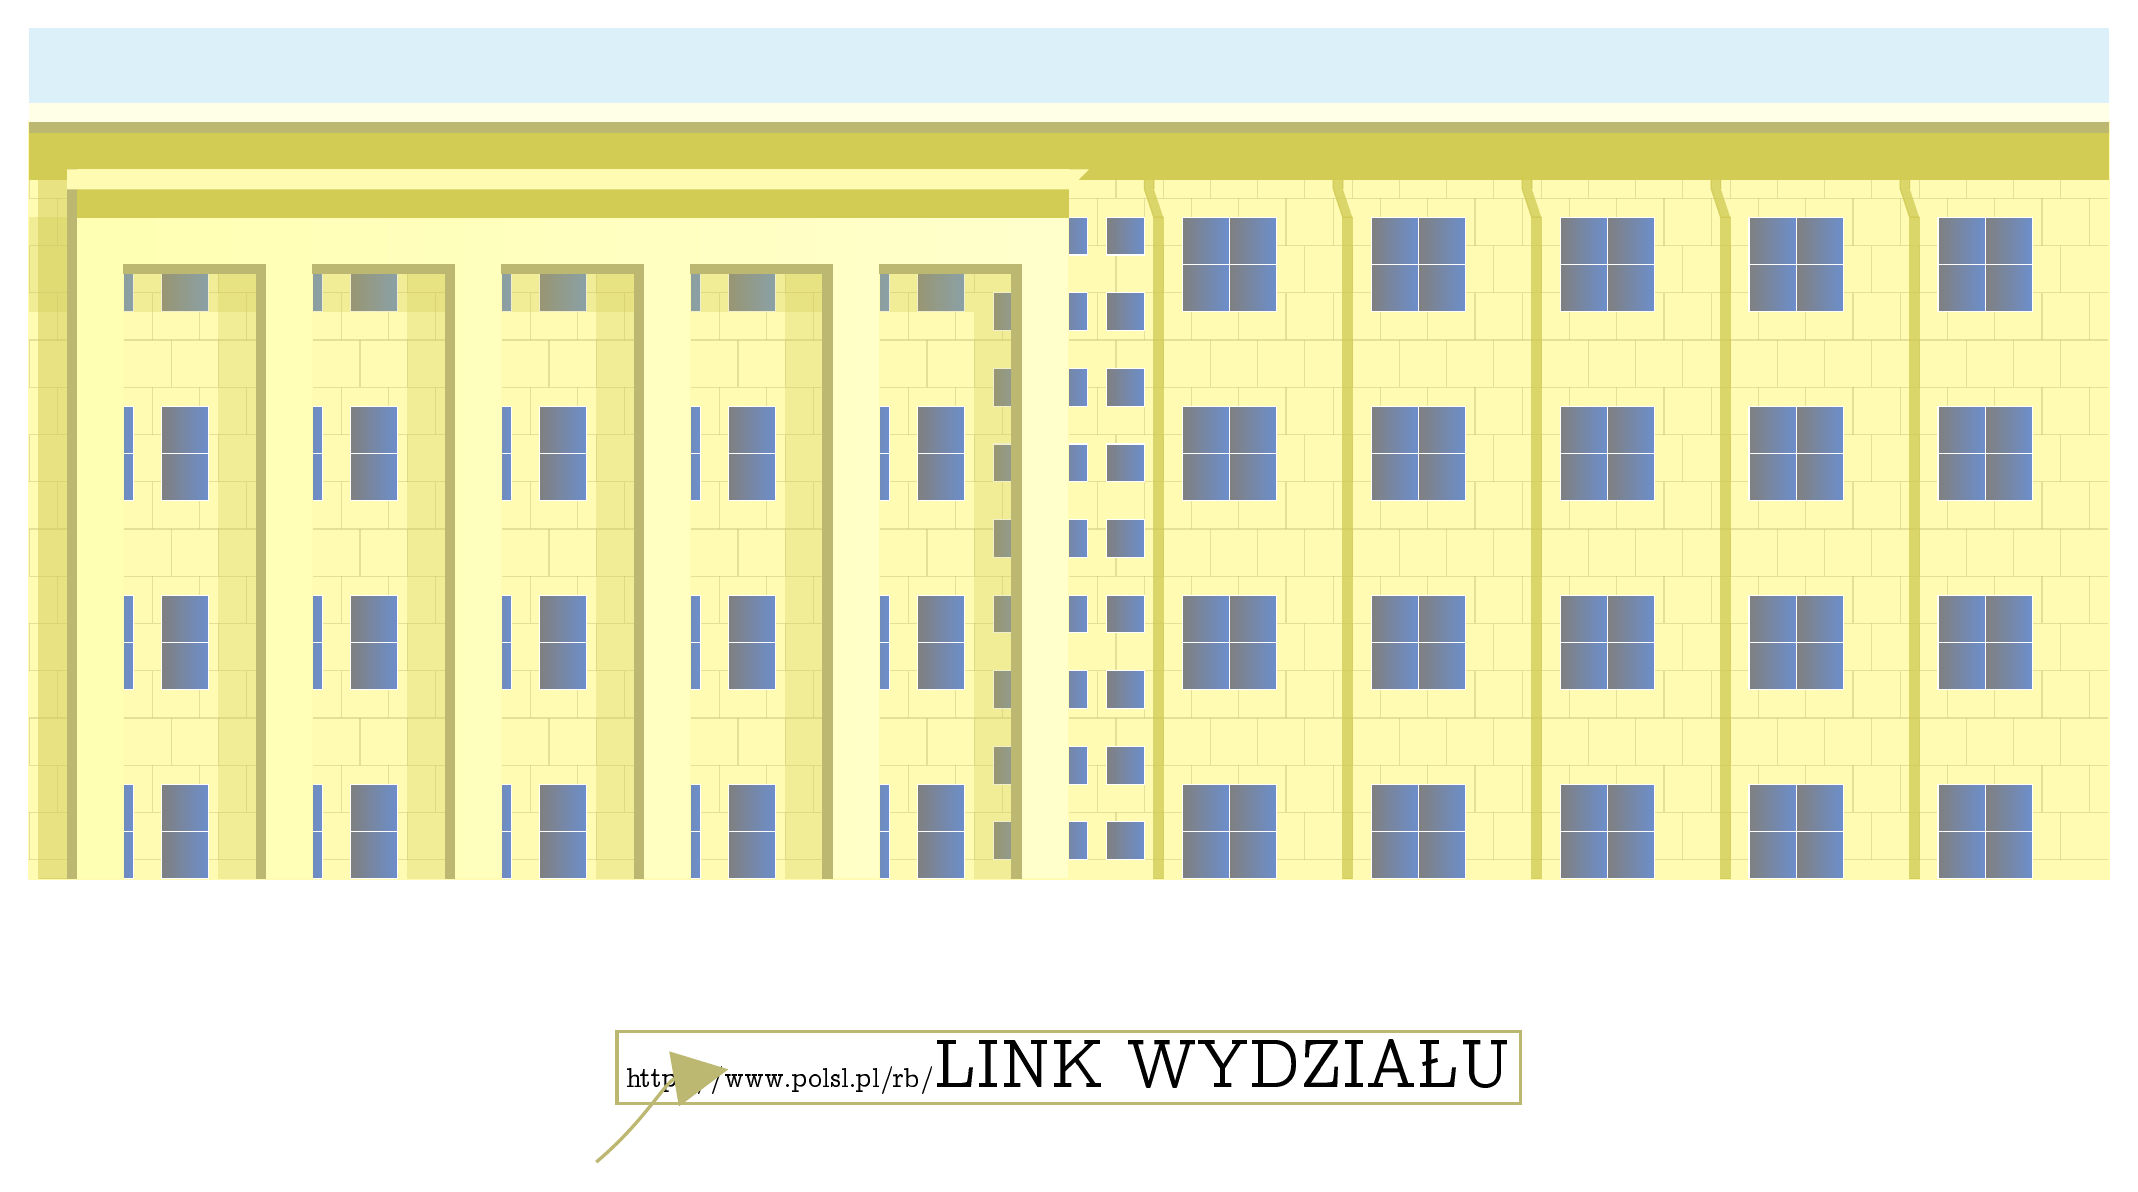
\begin{tikzpicture}[scale=1.2]
%\draw[help lines] (0,0) grid (21,10);
\filldraw[SkyBlue!30](0,1)rectangle(22,10);

\draw[yellow!30,fill=yellow!30,very thick] (0,1) to(0,9) to(22,9) to (22,1) to(0,1);

%%%% wzór kostki %%%%
\foreach \j in {1,...,8}
{\draw[yellow!40!gray,opacity=0.4](0,\j+0.7)to(22,\j+0.7);
\draw[yellow!40!gray,opacity=0.4](0,\j+0.2)to(22,\j+0.2);
\foreach \i in {0,0.5,1,1.5,...,21.5}{
\draw[yellow!40!gray,opacity=0.4](\i,\j+0.2)to(\i,\j+0.7);
\draw[yellow!40!gray,opacity=0.4](\i+0.3,\j+0.7)to(\i+0.3,\j+1.2);
}
}

%%%% okna %%%%

\foreach \j in {1,2,3,4}{
\foreach \i in {0,...,4}{
\filldraw[White,left color=gray, right color=gray!30!CornflowerBlue] (2*\i+0.6, 2*\j-1) rectangle (2*\i+1.1, 2*\j);
\filldraw[White,left color=gray, right color=gray!30!CornflowerBlue] (2*\i+1.4, 2*\j-1) rectangle (2*\i+1.9, 2*\j);
\draw[White](2*\i+0.6, 2*\j-0.5)to(2*\i+1.1, 2*\j-0.5);
\draw[White](2*\i+1.4, 2*\j-0.5)to(2*\i+1.9, 2*\j-0.5);
}

\foreach \i in {6,...,10}{
\filldraw[White,left color=gray, right color=gray!30!CornflowerBlue] (2*\i+0.2, 2*\j-1) rectangle (2*\i+0.7, 2*\j);
\filldraw[White,left color=gray, right color=gray!30!CornflowerBlue] (2*\i+0.7, 2*\j-1) rectangle (2*\i+1.2, 2*\j);
\draw[White](2*\i+0.2, 2*\j-0.5)to(2*\i+1.2, 2*\j-0.5);

%%%% rynny %%%%

\filldraw[yellow!60!gray,opacity=0.3](2*\i, 1) rectangle (2*\i-0.1, 8);
\filldraw[yellow!60!gray,opacity=0.3](2*\i, 8)to(2*\i-0.1,8)to(2*\i-0.2, 8.3)to(2*\i-0.2, 8.5)to(2*\i-0.1, 8.5)to(2*\i-0.1, 8.3);
}}



%%%% małe okienka %%%%
\foreach \j in {2,...,10}{
\foreach \i in {17,...,19}{
\filldraw[White,left color=gray, right color=gray!30!CornflowerBlue] (0.6*\i, 0.8*\j-0.4)rectangle (0.6*\i+0.4, 0.8*\j);
}
}

%%%% dach %%%%
\filldraw[yellow!60!gray](0,8.4)rectangle(22,8.9);
\filldraw[yellow!10](0,9)rectangle(22,9.2);
\filldraw[yellow!40!gray](0,8.9)rectangle(22,9);

\foreach \i in {-1,0,1,2,3}{
\filldraw[draw=none,opacity=0.3,fill=yellow!60!gray,fill opacity=0.3](2*\i+4,1)rectangle(2*\i+4.7,8);
\filldraw[draw=none,opacity=0.3,fill=yellow!60!gray,fill opacity=0.3](2*\i+2,7)rectangle(2*\i+4,8);
}

%%%% front %%%%
\filldraw[yellow!30,left color=yellow!30, right color=yellow!20](0.5,1)to(0.5,8.5)to(11,8.5)to(11,1)to(10.5,1)to(10.5,7.5)to(9,7.5)to(9,1)to(8.5,1)to(8.5,7.5)to(7,7.5)to(7,1)to(6.5,1)to(6.5,7.5)to(5,7.5)to(5,1)to(4.5,1)to(4.5,7.5)to(3,7.5)to(3,1)to(2.5,1)to(2.5,7.5)to(1,7.5)to(1,1)to(0.5,1)to(0.5,8.5);


%%%% cienie %%%%

\filldraw[yellow!60!gray,opacity=0.5](0.1,1)rectangle(0.5,8.7);
\filldraw[yellow!60!gray](0.5,8.3)to(11,8.3)to(11,8)to(0.5,8);


\filldraw[yellow!40!gray](0.5,1)to(0.5,8.5)to(0.4,8.5)to(0.4,1);

\filldraw[yellow!30](0.4,8.3)to(11,8.3)to(11.2,8.5)to(0.4,8.5);

\filldraw[yellow!40!gray](2.5,1)to(2.5,7.5)to(2.4,7.5)to(2.4,1);
\filldraw[yellow!40!gray](4.5,1)to(4.5,7.5)to(4.4,7.5)to(4.4,1);
\filldraw[yellow!40!gray](6.5,1)to(6.5,7.5)to(6.4,7.5)to(6.4,1);
\filldraw[yellow!40!gray](8.5,1)to(8.5,7.5)to(8.4,7.5)to(8.4,1);
\filldraw[yellow!40!gray](10.5,1)to(10.5,7.5)to(10.4,7.5)to(10.4,1);
\filldraw[yellow!40!gray](10.5,7.5)to(9,7.5)to(9,7.4)to(10.5,7.4);
\filldraw[yellow!40!gray](8.5,7.5)to(7,7.5)to(7,7.4)to(8.5,7.4);
\filldraw[yellow!40!gray](6.5,7.5)to(5,7.5)to(5,7.4)to(6.5,7.4);
\filldraw[yellow!40!gray](4.5,7.5)to(3,7.5)to(3,7.4)to(4.5,7.4);
\filldraw[yellow!40!gray](2.5,7.5)to(1,7.5)to(1,7.4)to(2.5,7.4);

%%%% odnośnik %%%%

\node [draw=yellow!40!gray,very thick] at (11,-1) {\href{https://www.polsl.pl/rb/}{\Huge{LINK WYDZIAŁU}}};
\node[draw=none] (A) at(7.5,-1){};
\draw [-{Triangle[length=7mm, width=7mm]},very thick,draw=yellow!40!gray] (6,-2) to [out=40,in=-170] (A);

\end{tikzpicture}

%%%%%%%%%%%%%%%%%%%%%%%%%%% RIF %%%%%%%%%%%%%%%%%%%%%%%%%%%%%%
\newpage
\centering\hypertarget{rb}{{\Huge{RIF}}}

\vspace{2cm}

\begin{tikzpicture}[scale=1.2]
%\draw[help lines] (0,0) grid (21,10);
\filldraw[SkyBlue!30](0,1)rectangle(22,10);

\filldraw[gray!30,very thick] (0,1) to(0,7) to[out=10,in=-180](22,9) to (22,1) to(0,1);

\draw[left color=gray!30,black,right color=SkyBlue!50!gray] (0,1) to(0,6) to[out=10,in=-180](22,8) to (22,1) to(0,1);

%%%% cienie okien %%%%
\foreach \j in {-1,0,1,...,18}{
\draw[gray!50!black,very thick](2.8+\j-1,1)to(2.8+\j-1,7+0.09*\j);
\filldraw[gray!50!black,very thick](2.5+\j,1)rectangle(2.6+\j,7+0.09*\j);}
\filldraw[gray!30] (0,6.1) to(0,7) to[out=10,in=-180](22,9) to (22,8.1)to[out=-180,in=10](0,6.1);
\filldraw[gray!50!black] (0,6) to(0,6.1) to[out=10,in=-180](22,8.1) to (22,8)to[out=-180,in=10](0,6);

%%%% poziome pasy %%%%
\filldraw[gray!90,very thick] (0,4) to(0,5) to[out=10,in=-180](22,7) to (22,6) to[out=180,in=10](0,4);
\draw[black!90,very thick](0,5.5) to[out=10,in=-180](22,7.4) ;
\filldraw[gray!90,very thick] (0,2) to(0,3) to[out=10,in=-180](22,5) to (22,4) to[out=180,in=10](0,2);
\draw[black!90,very thick](0,3.5) to[out=10,in=-180](22,5.4);
\filldraw[gray!90,very thick](0,1) to[out=10,in=-180](22,3) to (22,2) to[out=180,in=10](5,1);
\draw[black!90,very thick](0,1.5) to[out=10,in=-180](22,3.4);

%%%% pionowe filary %%%%
\foreach \j in {-1,0,1,...,18}{
\filldraw[gray!30,very thick](2+\j,1)rectangle(2.5+\j,7+0.1*\j);
}

%%%% cień %%%%
\draw[left color=CadetBlue!30,CadetBlue!30,right color=CadetBlue!70!gray!70!Periwinkle,very thick,fill opacity=0.6] (0,1) to(0,7) to[out=10,in=-180](22,9) to (22,1) to(0,1);

%%%% linia dach %%%%
\draw[black!70!gray,very thin](0,6.5) to[out=10,in=-180](22,8.5);

%%%% odnośnik %%%%
\node [draw=gray,very thick] at (11,-1) {\href{https://www.polsl.pl/rif/}{\Huge{LINK WYDZIAŁU}}};
\node[draw=none] (A) at(7.5,-1){};
\draw [-{Triangle[length=7mm, width=7mm]},very thick,draw=gray] (6,-2) to [out=40,in=-170] (A);
\end{tikzpicture}


%%%%%%%%%%%%%%%%%%%%%%%%%%% RAR %%%%%%%%%%%%%%%%%%%%%%%%%%%%%%
\newpage
\centering\hypertarget{rb}{{\Huge{RAR}}}

\vspace{2cm}
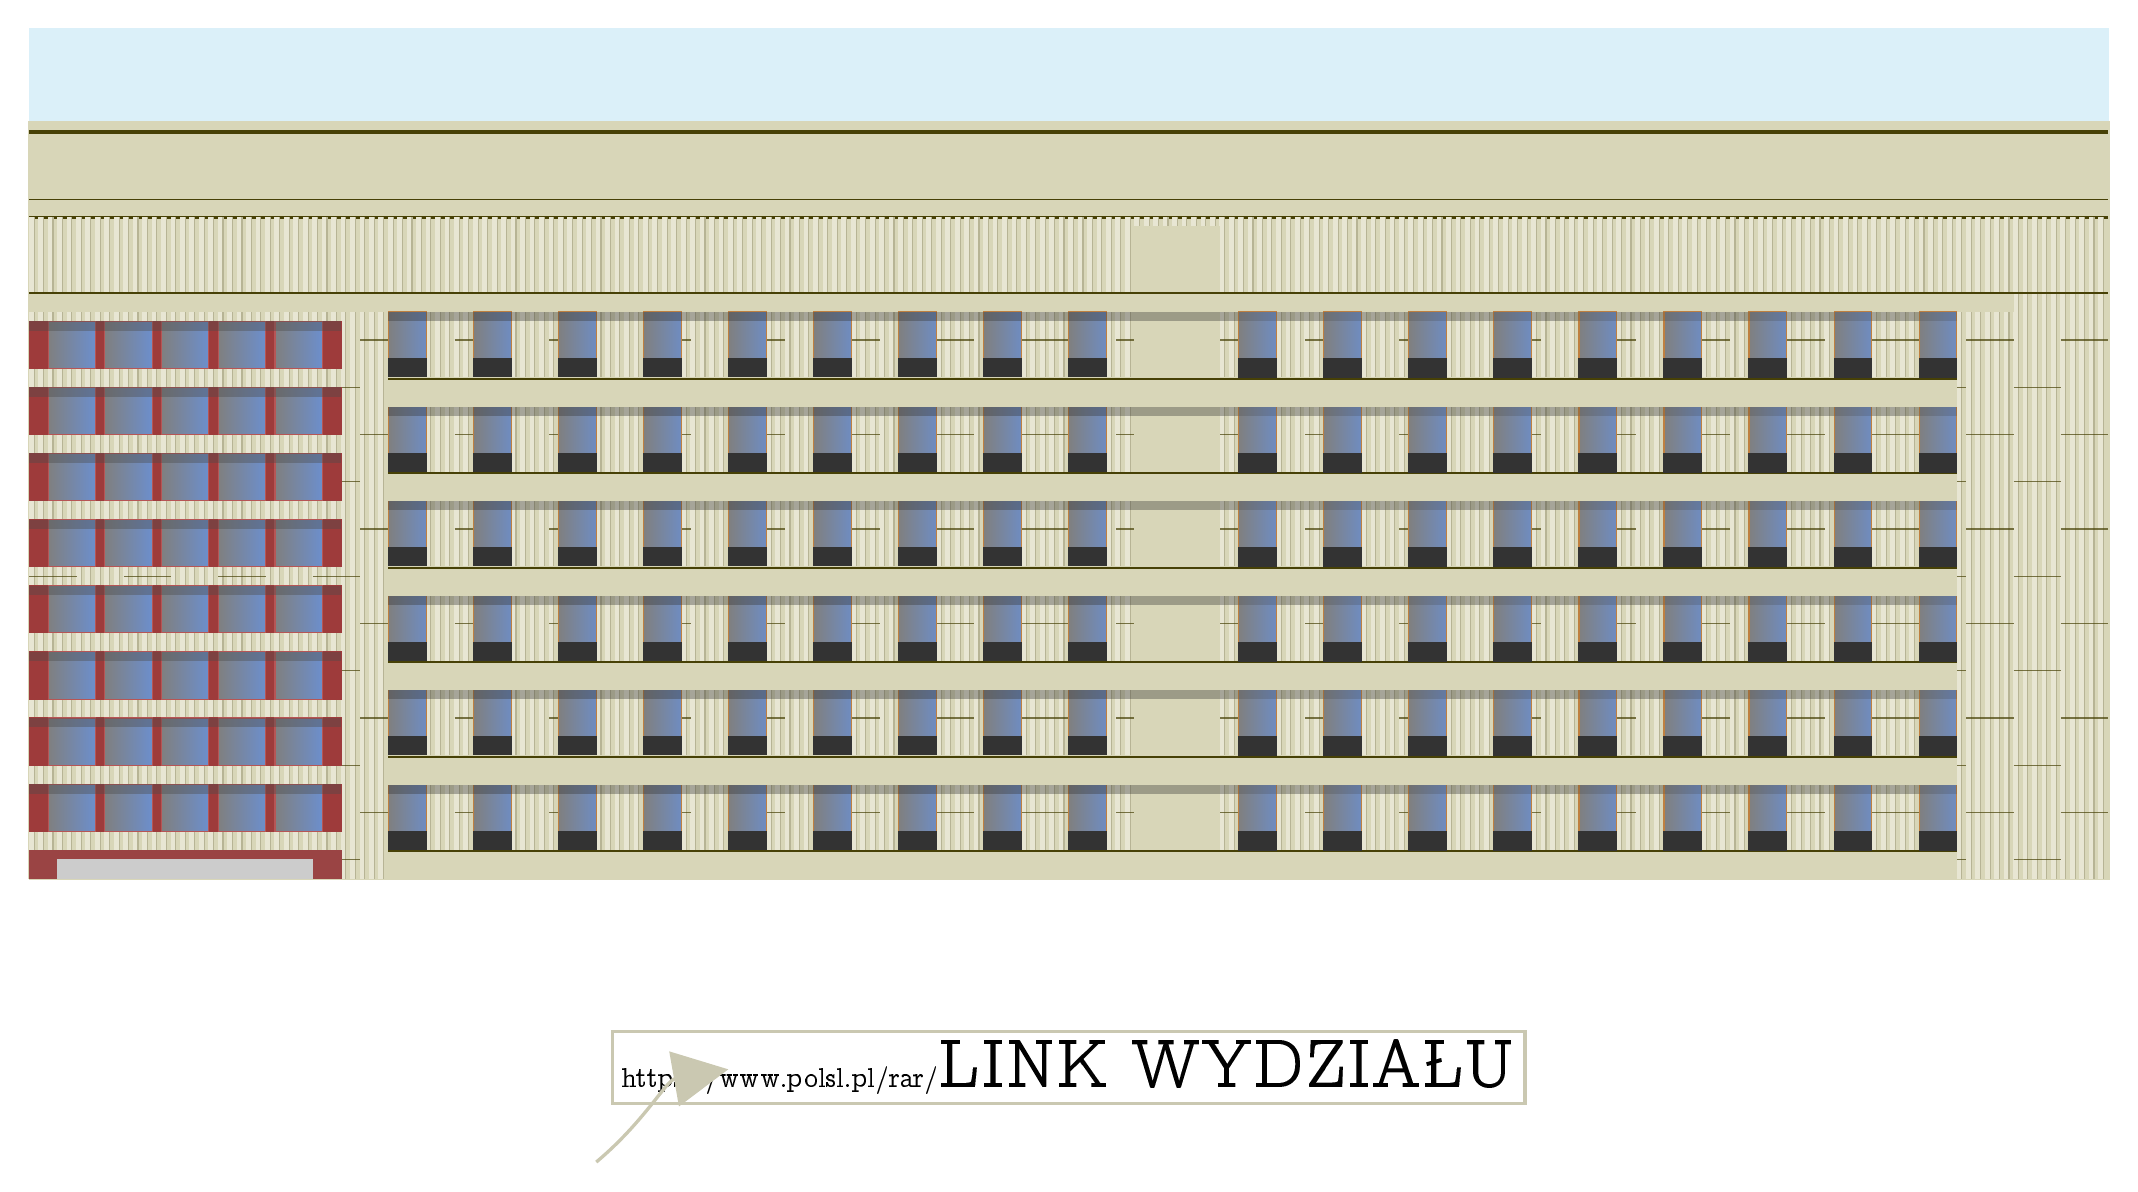
\begin{tikzpicture}[scale=1.2]
%\draw[help lines] (0,0) grid (21,10);
\filldraw[SkyBlue!30](0,1)rectangle(22,10);
\draw[gray!70!yellow!50,fill=gray!70!yellow!50,very thick] (0,1) to(0,9) to(22,9) to (22,1) to(0,1);
%%%% dach %%%%
\draw[brown!30!yellow!30!black,very thick](0,8.9)to(22,8.9);
\draw[brown!30!yellow!30!black,very thick](0,8)to(22,8);
\draw[brown!30!yellow!30!black,very thick](0,8.2)to(22,8.2);

%%%% paski pion %%%%
\foreach \i in {0,1,...,219}{
\filldraw[gray!70!yellow!30]((0.1*\i, 1) rectangle (0.1*\i+0.05, 8);
\draw[brown!30!yellow!30!black,opacity=0.3]((0.1*\i+0.05, 1) to (0.1*\i+0.05, 8);
}
%%%% paski poziom %%%%
\foreach \j in {1,...,6}{
\foreach \i in {0,...,21}
{
\draw[brown!30!yellow!30!black,opacity=0.7,thin](\i,\j+0.2)to(\i+0.5,\j+0.2);
\draw[brown!30!yellow!30!black,opacity=0.7,thin](\i+0.5,\j+0.7)to(\i+1,\j+0.7);
}}

\filldraw[gray!70!yellow!50](11.7,1)rectangle(12.6,7.9);
\filldraw[gray!70!yellow!50](0,7)rectangle(21,7.2);
\draw[brown!30!yellow!30!black,thick](0,7.2)to(22,7.2);
\filldraw[gray!70!yellow!50](0,8.2)rectangle(22,8.7);
%%%% okna %%%%
\foreach \k in {0,9}{
\foreach \j in {1,2,...,6}{

\filldraw[gray!70!yellow!50](3.8,\j+0.3)rectangle(20.4,\j);
\draw[brown!30!yellow!30!black, thick](3.8,\j+0.29)to(20.4,\j+0.29);

\foreach \i in {4,...,12}{
\filldraw[brown,left color=gray, right color=gray!40!CornflowerBlue] (\k+0.9*\i+0.2, \j+0.3) rectangle (\k+0.9*\i+0.6, \j+1);

\filldraw[Black!80] (\k+0.9*\i+0.2, \j+0.3) rectangle (\k+0.9*\i+0.6, \j+0.5);
}
\filldraw[draw=none,black!80,opacity=0.2](3.8,\j+1)rectangle(20.4,\j+0.9);

}}


%%%% okna małe %%%%
\foreach \j in {1,2,...,8}{
\filldraw[Brown!80!gray](0,0.7*\j+0.8)rectangle(3.3,0.7*\j+1.3);

\foreach \i in {0,...,4}{
\filldraw[Brown!80,left color=gray, right color=gray!30!CornflowerBlue] (0.6*\i+0.2, 0.7*\j+0.8) rectangle (0.6*\i+0.7, 0.7*\j+1.3);
}
\filldraw[draw=none,black!70,opacity=0.4](0,0.7*\j+1.2)rectangle(3.3,0.7*\j+1.3);}
\filldraw[Brown!70!gray](0,1)rectangle(3.3,1.3);
\filldraw[white!60!gray](0.3,1)rectangle(3,1.2);

%%%% odnośnik %%%%
\node [draw=gray!80!yellow!60,very thick] at (11,-1) {\href{https://www.polsl.pl/rar/}{\Huge{LINK WYDZIAŁU}}};

\node[draw=none] (A) at(7.5,-1){};
\draw [-{Triangle[length=7mm, width=7mm]},very thick,draw=gray!80!yellow!60] (6,-2) to [out=40,in=-170] (A);
\end{tikzpicture}

%%%%%%%%%%%%%%%%%%%%%%%%%%% RIE %%%%%%%%%%%%%%%%%%%%%%%%%%%%%%

\newpage
\centering\hypertarget{rie}{{\Huge{RIE}}}

\vspace{2cm}
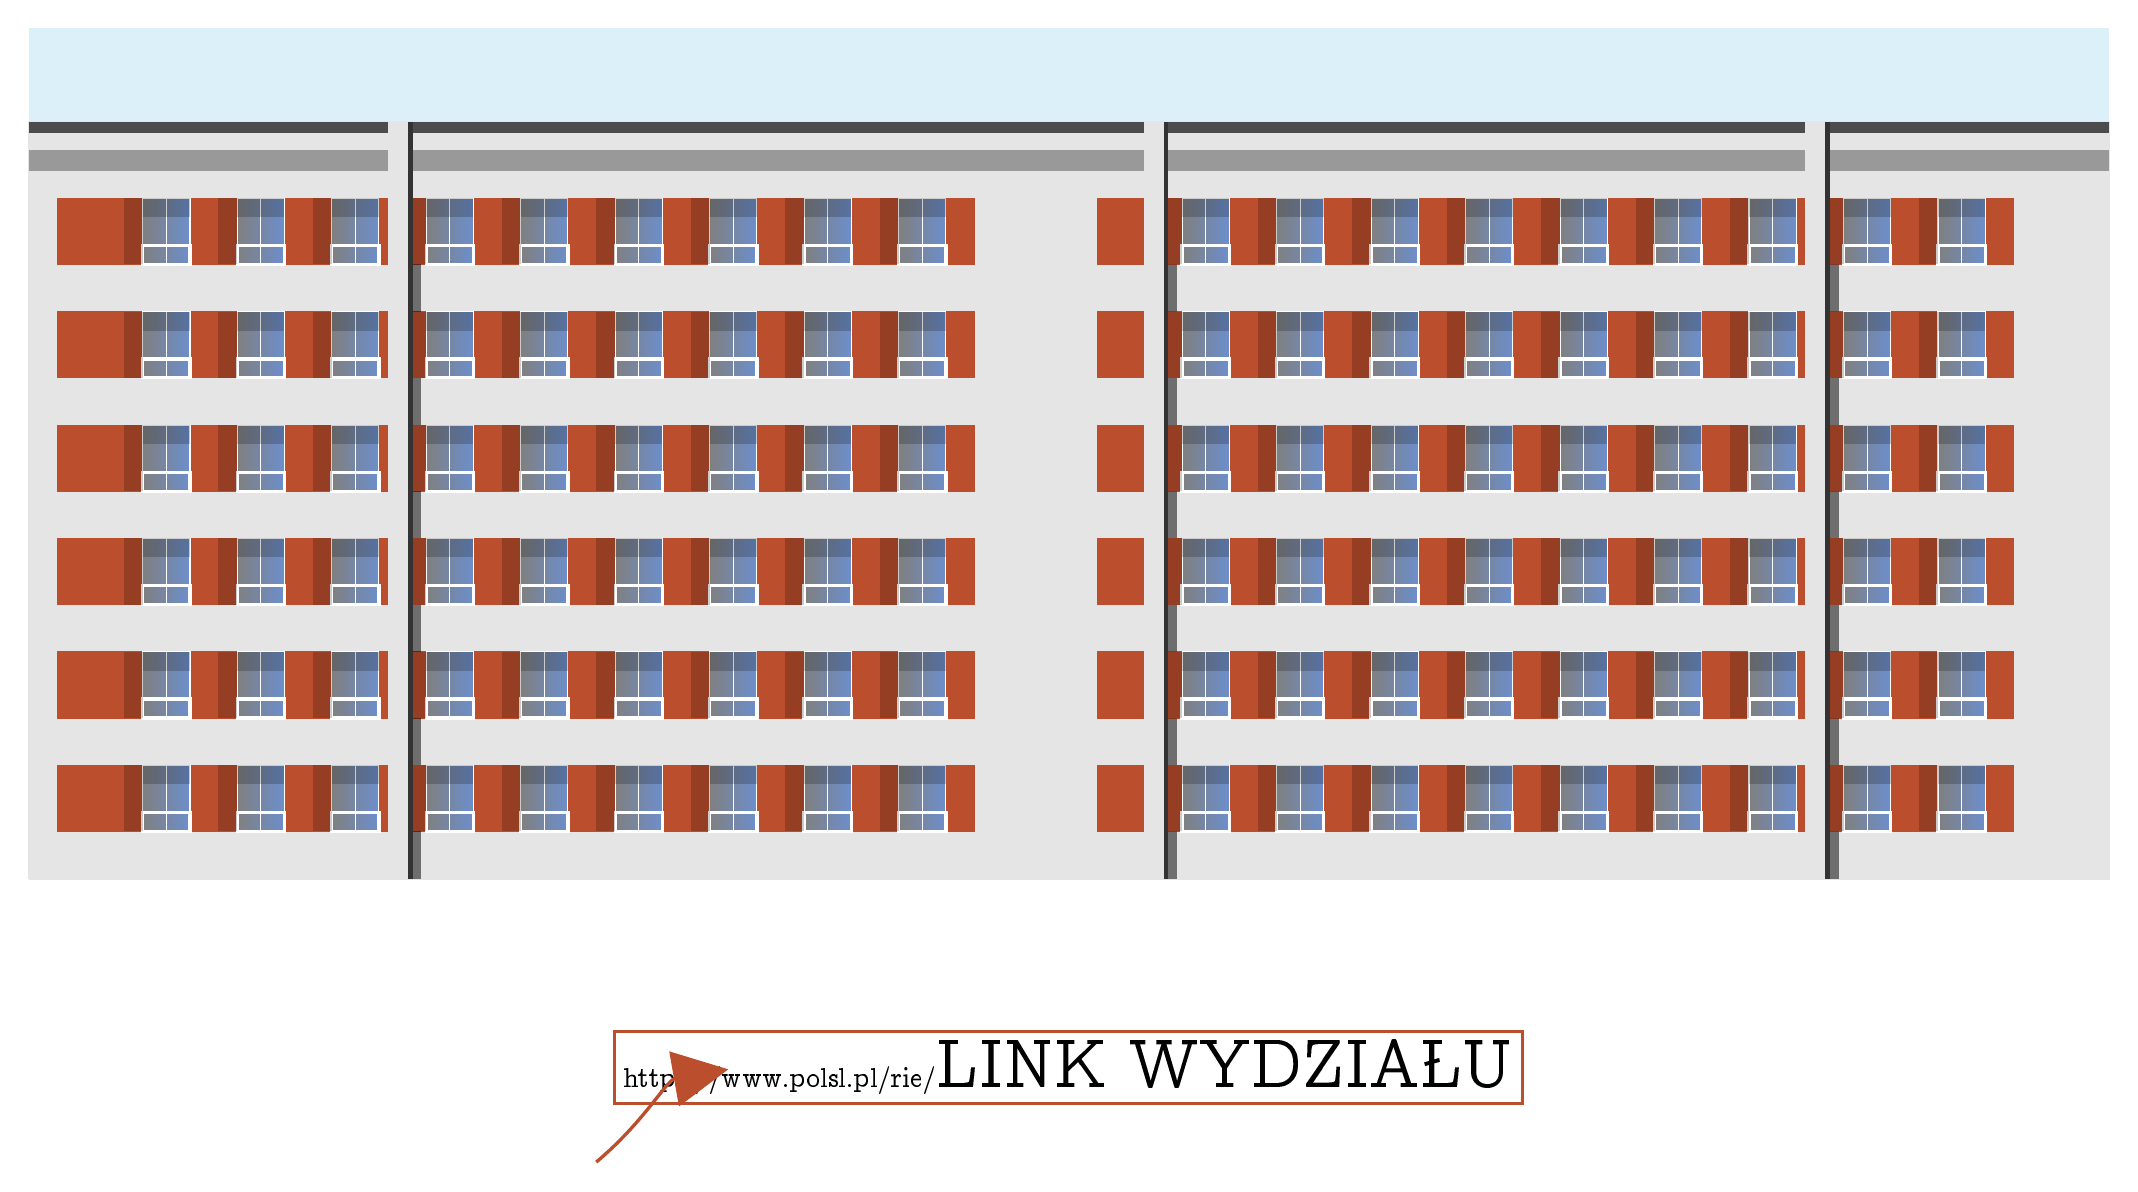
\begin{tikzpicture}[scale=1.2]
%\draw[help lines] (0,0) grid (21,10);
\filldraw[SkyBlue!30](0,1)rectangle(22,10);
\draw[gray!20,fill=gray!20,very thick] (0,1) to(0,9) to(22,9) to (22,1) to(0,1);

%%%% brąz i cienie %%%%
\foreach \k in {1,12}{
\foreach \j in {1,2,...,6}{
\filldraw[BrickRed!60!brown](\k-0.7, 1.2*\j+0.3)rectangle(\k+9, 1.2*\j+1);
\filldraw[draw=none,black,opacity=0.3](4.05, 1.2*\j-0.2)rectangle(4.15, 1.2*\j+0.3);
\filldraw[draw=none,black,opacity=0.3](12.05, 1.2*\j-0.2)rectangle(12.15,1.2*\j+0.3);
\filldraw[draw=none,black,opacity=0.3](19.05, 1.2*\j-0.2)rectangle(19.15,1.2*\j+0.3);

%%%% okna %%%%
\foreach \i in {0,...,8}{
\filldraw[white,left color=gray, right color=gray!30!CornflowerBlue] (\k+\i+0.2, 1.2*\j+0.3) rectangle (\k+\i+0.7, 1.2*\j+1);
\filldraw[White,left color=gray, right color=gray!30!CornflowerBlue,very thick] (\k+\i+0.2, 1.2*\j+0.3) rectangle (\k+\i+0.7, 1.2*\j+0.5);
\draw[white] (\k+\i+0.45, 1.2*\j+0.3) rectangle (\k+\i+0.45, 1.2*\j+1);

\filldraw[draw=none,black,opacity=0.2] (\k+\i, 1.2*\j+0.3) rectangle (\k+\i+0.2, 1.2*\j+1);
\filldraw[draw=none,black,opacity=0.2](\k+\i+0.2, 1.2*\j+0.8) rectangle (\k+\i+0.7, 1.2*\j+1);
}}}


%%%% dach %%%%
\filldraw[gray!80](0,8.5)rectangle(22,8.7);
\filldraw[black!70](0,8.9)rectangle(22,9);

%%%% paski pion %%%%
\filldraw[black!80](4,1)rectangle(4.05,9);
\filldraw[black!80](12,1)rectangle(12.05,9);
\filldraw[black!80](19,1)rectangle(19.05,9);
\filldraw[gray!20](3.8,1)rectangle(4,9);
\filldraw[gray!20](11.8,1)rectangle(12,9);
\filldraw[gray!20](18.8,1)rectangle(19,9);

%%%% odnośnik %%%%

\node [draw=BrickRed!60!brown,very thick]at (11,-1) {\href{https://www.polsl.pl/rie/}{\Huge{LINK WYDZIAŁU}}};
\node[draw=none] (A) at(7.5,-1){};
\draw [-{Triangle[length=7mm, width=7mm]},very thick,draw=BrickRed!60!brown] (6,-2) to [out=40,in=-170] (A);
\end{tikzpicture}


%%%%%%%%%%%%%%%%%%%%%%%%%%% RMT %%%%%%%%%%%%%%%%%%%%%%%%%%%%%%


\newpage
\centering\hypertarget{rmt}{{\Huge{RMT}}}

\vspace{2cm}

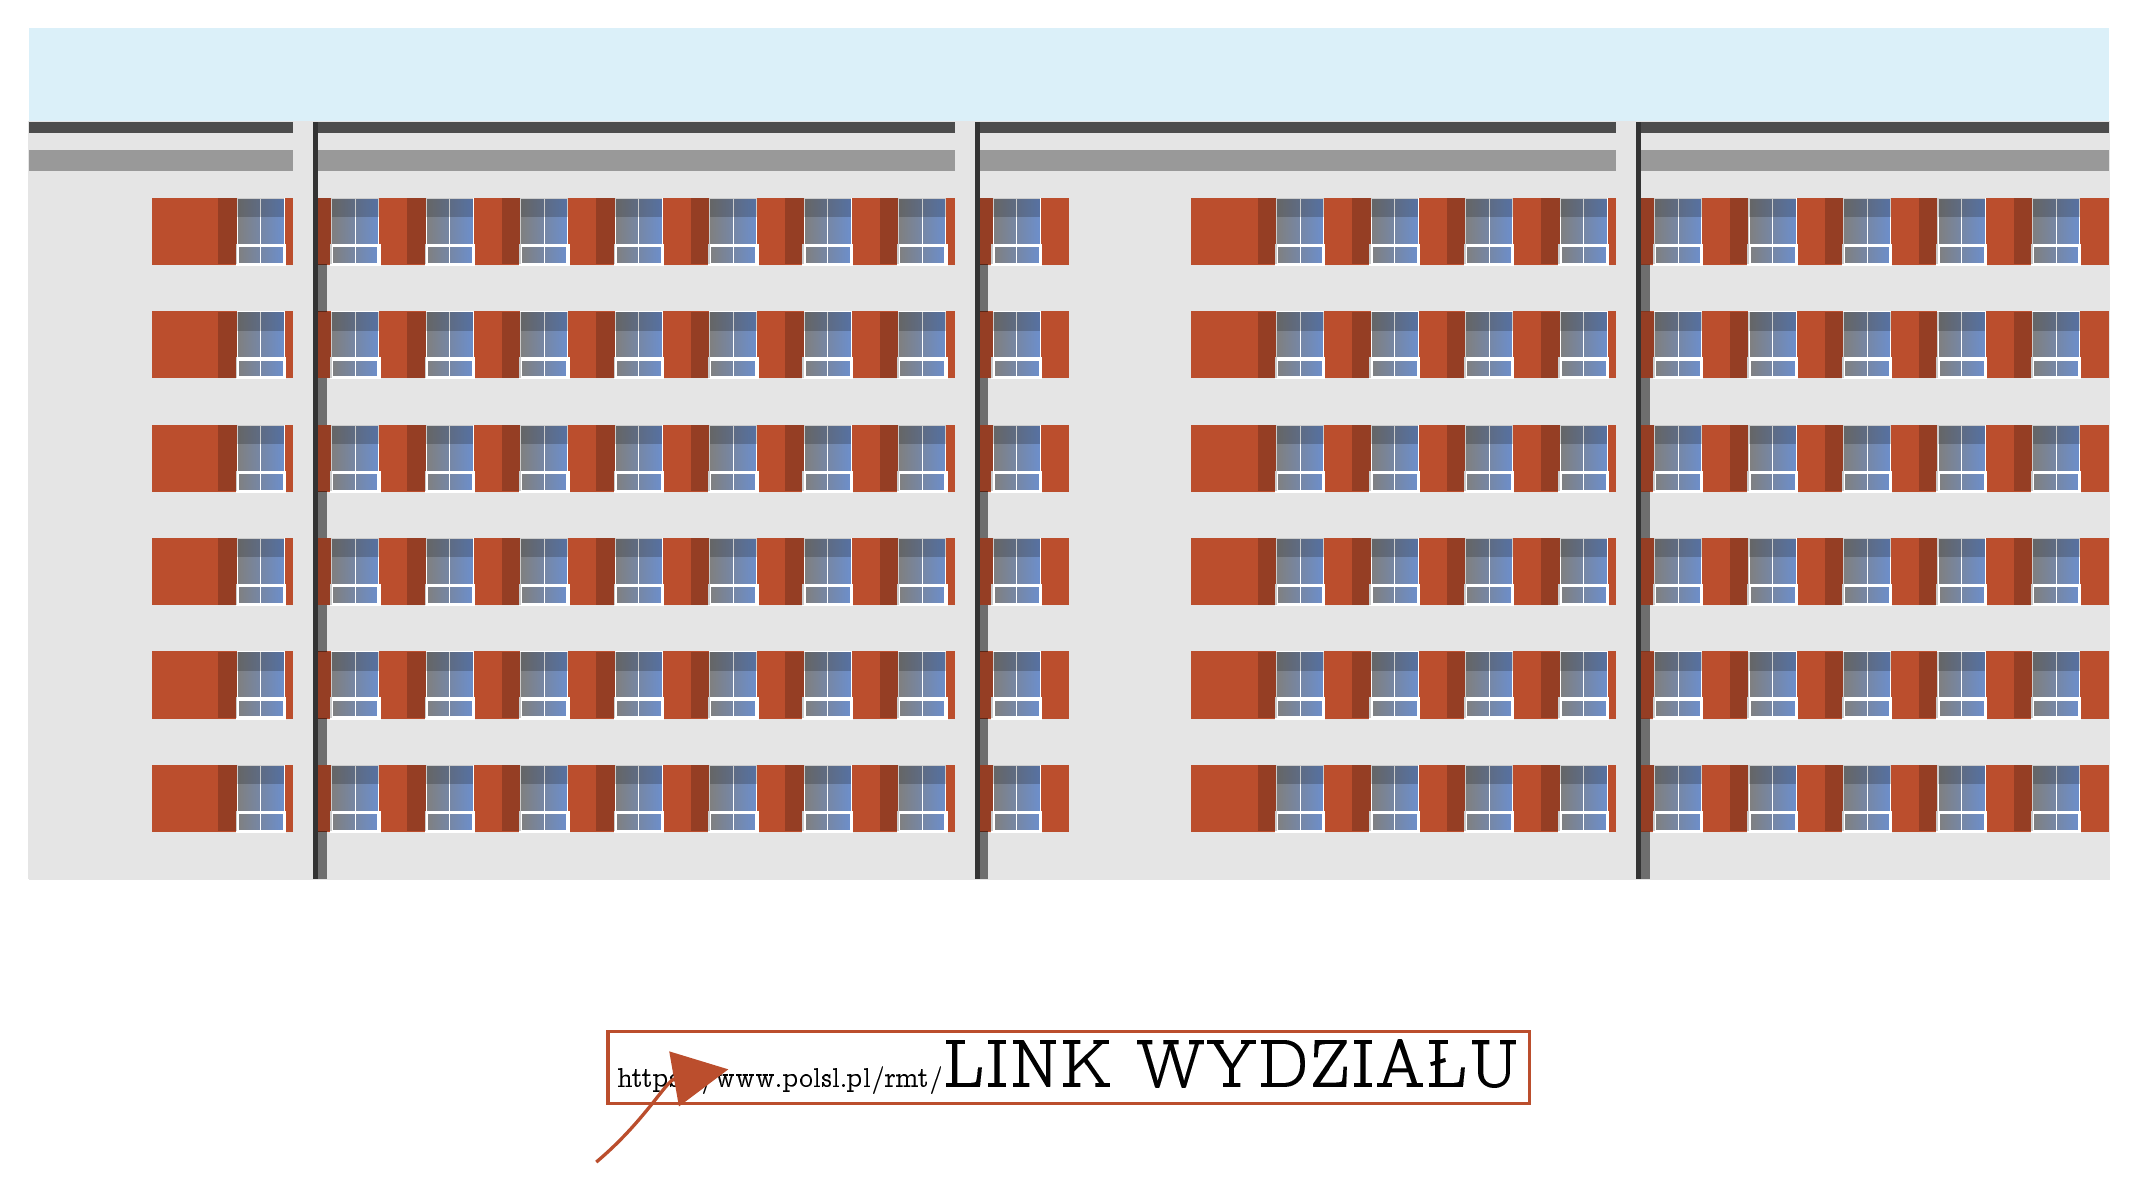
\begin{tikzpicture}[scale=1.2]
%\draw[help lines] (0,0) grid (21,10);
\filldraw[SkyBlue!30](0,1)rectangle(22,10);
\draw[gray!20,fill=gray!20,very thick] (0,1) to(0,9) to(22,9) to (22,1) to(0,1);

%%%% brąz i cienie %%%%
\foreach \k in {2,13}{
\foreach \j in {1,2,...,6}{
\filldraw[BrickRed!60!brown](\k-0.7, 1.2*\j+0.3)rectangle(\k+9, 1.2*\j+1);
\filldraw[draw=none,black,opacity=0.3](3.05, 1.2*\j-0.2)rectangle(3.15, 1.2*\j+0.3);
\filldraw[draw=none,black,opacity=0.3](10.05, 1.2*\j-0.2)rectangle(10.15,1.2*\j+0.3);
\filldraw[draw=none,black,opacity=0.3](17.05, 1.2*\j-0.2)rectangle(17.15,1.2*\j+0.3);

%%%% okna %%%%
\foreach \i in {0,...,8}{
\filldraw[white,left color=gray, right color=gray!30!CornflowerBlue] (\k+\i+0.2, 1.2*\j+0.3) rectangle (\k+\i+0.7, 1.2*\j+1);
\filldraw[White,left color=gray, right color=gray!30!CornflowerBlue,very thick] (\k+\i+0.2, 1.2*\j+0.3) rectangle (\k+\i+0.7, 1.2*\j+0.5);
\draw[white] (\k+\i+0.45, 1.2*\j+0.3) rectangle (\k+\i+0.45, 1.2*\j+1);

\filldraw[draw=none,black,opacity=0.2] (\k+\i, 1.2*\j+0.3) rectangle (\k+\i+0.2, 1.2*\j+1);
\filldraw[draw=none,black,opacity=0.2](\k+\i+0.2, 1.2*\j+0.8) rectangle (\k+\i+0.7, 1.2*\j+1);
}}}

%%%% dach %%%%
\filldraw[gray!80](0,8.5)rectangle(22,8.7);
\filldraw[black!70](0,8.9)rectangle(22,9);

%%%% paski pion %%%%
\filldraw[black!80](3,1)rectangle(3.05,9);
\filldraw[black!80](10,1)rectangle(10.05,9);
\filldraw[black!80](17,1)rectangle(17.05,9);
\filldraw[gray!20](2.8,1)rectangle(3,9);
\filldraw[gray!20](9.8,1)rectangle(10,9);
\filldraw[gray!20](16.8,1)rectangle(17,9);

%%%% odnośnik %%%%
\node [draw=BrickRed!60!brown,very thick] at (11,-1) {\href{https://www.polsl.pl/rmt/}{\Huge{LINK WYDZIAŁU}}};
\node[draw=none] (A) at(7.5,-1){};
\draw [-{Triangle[length=7mm, width=7mm]},very thick,draw=BrickRed!60!brown] (6,-2) to [out=40,in=-170] (A);
\end{tikzpicture}


%%%%%%%%%%%%%%%%%%%%%%%%%%% RE %%%%%%%%%%%%%%%%%%%%%%%%%%%%%%
\newpage
\centering\hypertarget{re}{{\Huge{RE}}}

\vspace{2cm}

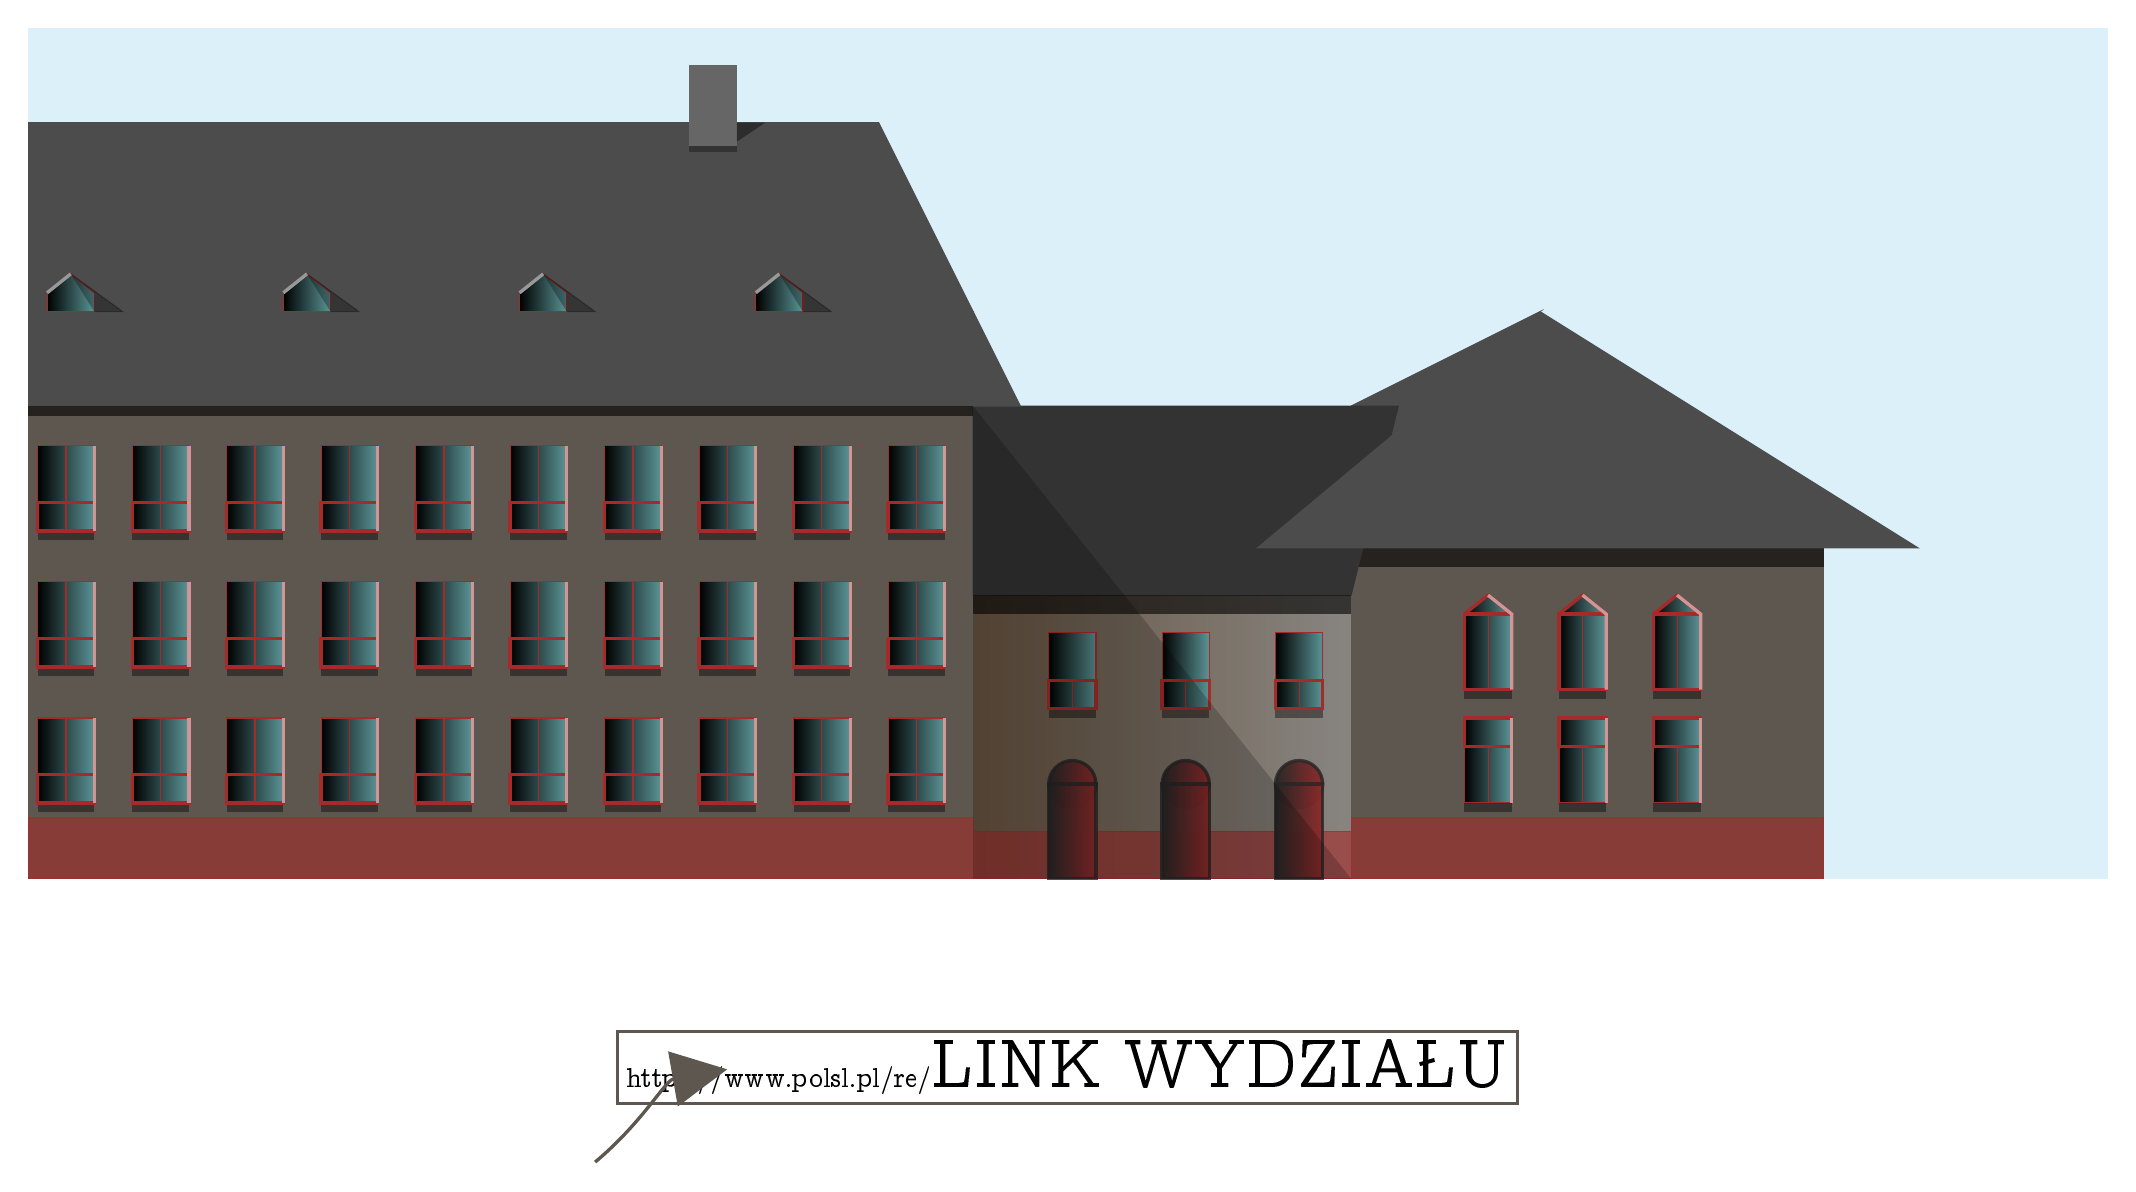
\begin{tikzpicture}[scale=1.2]
%\draw[help lines] (0,0) grid (21,10);
\filldraw[SkyBlue!30](0,1)rectangle(22,10);

\filldraw[darkgray!90!Tan,left color=darkgray!70!brown,right color=gray!90!Tan](10,1)rectangle(14,5);


%%%% budynki, dach i paski %%%%

\filldraw[Brown,opacity=0.6](10,1)rectangle(14,1.5);
\filldraw[darkgray!80!Tan](0,1)rectangle(10,7);
\filldraw[Brown,opacity=0.6](0,1)rectangle(10,1.65);
\filldraw[darkgray!80!Tan](14,1)rectangle(19,5);
\filldraw[Brown,opacity=0.6](14,1)rectangle(19,1.65);
\filldraw[black!70](13,4.5)to(16,7)to(14,6);
\filldraw[black,draw=none,opacity=0.6](14,4.3)rectangle(19,4.5);
\filldraw[black!80](10,4)to(10,6)to(14.5,6)to(14,4)to(10,4);
\filldraw[black!70](13,4.5)to(20,4.5)to(16,7);
\filldraw[black!70](0,6)to(10.5,6)to(9,9)to(0,9);
\filldraw[black,draw=none,opacity=0.6](10,3.8)rectangle(14,4);
\filldraw[black,draw=none,opacity=0.6](0,5.9)rectangle(10,6);
\filldraw[black!60](7,8.7)rectangle(7.5,9.6);
\filldraw[black!80](7,8.7)rectangle(7.5,8.75);
\filldraw[draw=none,black,opacity=0.4](7.5,8.8)to(7.8,9)to(7.5,9);


%%%% okna nad drzwiami %%%%
\foreach \i in {9,10,11}{
\filldraw[Brown,left color=Black, right color=darkgray!10!CadetBlue] (1.2*\i, 2.8) rectangle (1.2*\i+0.5, 3.6);
\filldraw[draw=none,black,opacity=0.4](1.2*\i, 2.8) rectangle (1.2*\i+0.5, 2.7);
\filldraw[Brown,left color=Black, right color=darkgray!10!CadetBlue,very thick] (1.2*\i,2.8) rectangle (1.2*\i+0.5, 3.1);


%%%% drzwi %%%%
\draw[Brown](1.2*\i+0.25,2.8)to(1.2*\i+0.25,3.1);
\filldraw[black!70!gray,left color=black!70!gray,right color=Brown,opacity=0.8,very thick] (1.2*\i+0.25,2) circle(0.25);
\filldraw[black!70!gray,left color=black!70!gray,right color=Brown,opacity=0.8,very thick] (1.2*\i,1) rectangle (1.2*\i+0.5, 2);
}

%%%% cień środek %%%%
\filldraw[draw=none,black,opacity=0.3,fill opacity=0.2](10,6)to(14,1)to(10,1);

%%%% okna lewo %%%%

\foreach \j in {1,1.9,2.8}{
\foreach \i in {0,...,9}{
\filldraw[Brown,left color=Black, right color=darkgray!10!CadetBlue] (\i+0.1, 1.6*\j+0.2) rectangle (\i+0.7, 1.6*\j+1.1);
\filldraw[draw=none,black,opacity=0.4] (\i+0.1, 1.6*\j+0.2) rectangle(\i+0.7, 1.6*\j+0.1);
\filldraw[Brown,left color=Black, right color=darkgray!10!CadetBlue,very thick] (\i+0.1, 1.6*\j+0.2) rectangle (\i+0.7, 1.6*\j+0.5);
\draw[Brown](\i+0.4,1.6*\j+0.2)to(\i+0.4,1.6*\j+1.1);
\draw[Brown!50,very thick](\i+0.7, 1.6*\j+1.1)to(\i+0.7, 1.6*\j+0.2);
}}
%%%% okienka dach %%%%
\foreach \j in {0,2.5,5,7.5}{

\filldraw[Brown,left color=Black, right color=darkgray!10!CadetBlue] (\j+0.2,7) rectangle (\j+0.7, 7.2);
\filldraw[Brown,left color=Black, right color=darkgray!10!CadetBlue] (\j+0.2,7.2) to(\j+0.45,7.4)to(\j+0.7, 7.2);
\filldraw[Black,opacity=0.3](\j+0.7,7)to(\j+1,7)to(\j+0.45,7.4);
\draw[Gray!80,very thick](\j+0.2,7.2) to(\j+0.45,7.4);
}

%%%% okna prawo %%%%
\foreach \i in {15,16,17}{
\filldraw[Brown,left color=Black, right color=darkgray!10!CadetBlue] (\i+0.2, 2.7) rectangle (\i+0.7, 1.8);
\filldraw[draw=none, black,opacity=0.4](\i+0.2, 1.7) rectangle (\i+0.7, 1.8);
\filldraw[Brown,left color=Black, right color=darkgray!10!CadetBlue,very thick] (\i+0.2, 1.6*1.5) rectangle (\i+0.7, 2.7);
\filldraw[draw=none, black,opacity=0.4](\i+0.2, 2.9) rectangle (\i+0.7, 3);
\filldraw[Brown,left color=Black, right color=darkgray!10!CadetBlue,very thick] (\i+0.2, 3.8) to(\i+0.45, 4)to (\i+0.7, 3.8);
\draw[Brown](\i+0.45,1.6*1.5)to(\i+0.45,1.8);
\draw[Brown!50,very thick](\i+0.7, 2.7)to (\i+0.7, 1.8);

\filldraw[Brown,left color=Black, right color=darkgray!10!CadetBlue] (\i+0.2, 3) rectangle (\i+0.7, 3.8);
\filldraw[Brown,left color=Black, right color=darkgray!10!CadetBlue,very thick] (\i+0.2, 3) rectangle (\i+0.7, 3.8);
\draw[Brown](\i+0.45,3)to(\i+0.45,3.8);
\draw[Brown!50,very thick](\i+0.45, 4)to(\i+0.7, 3.8)to (\i+0.7, 3);
}

%%%% odnośnik %%%%
\node [draw=darkgray!80!Tan,very thick]at (11,-1) {\href{https://www.polsl.pl/re/}{\Huge{LINK WYDZIAŁU}}};
\node[draw=none] (A) at(7.5,-1){};
\draw [-{Triangle[length=7mm, width=7mm]},very thick,draw=darkgray!80!Tan] (6,-2) to [out=40,in=-170] (A);
\end{tikzpicture}

%%%%%%%%%%%%%%%%%%%%%%%%% RMS %%%%%%%%%%%%%%%%%%%%%%%%%%%%%%5
\newpage
\centering\hypertarget{rms}{{\Huge{RMS}}}

\vspace{2cm}
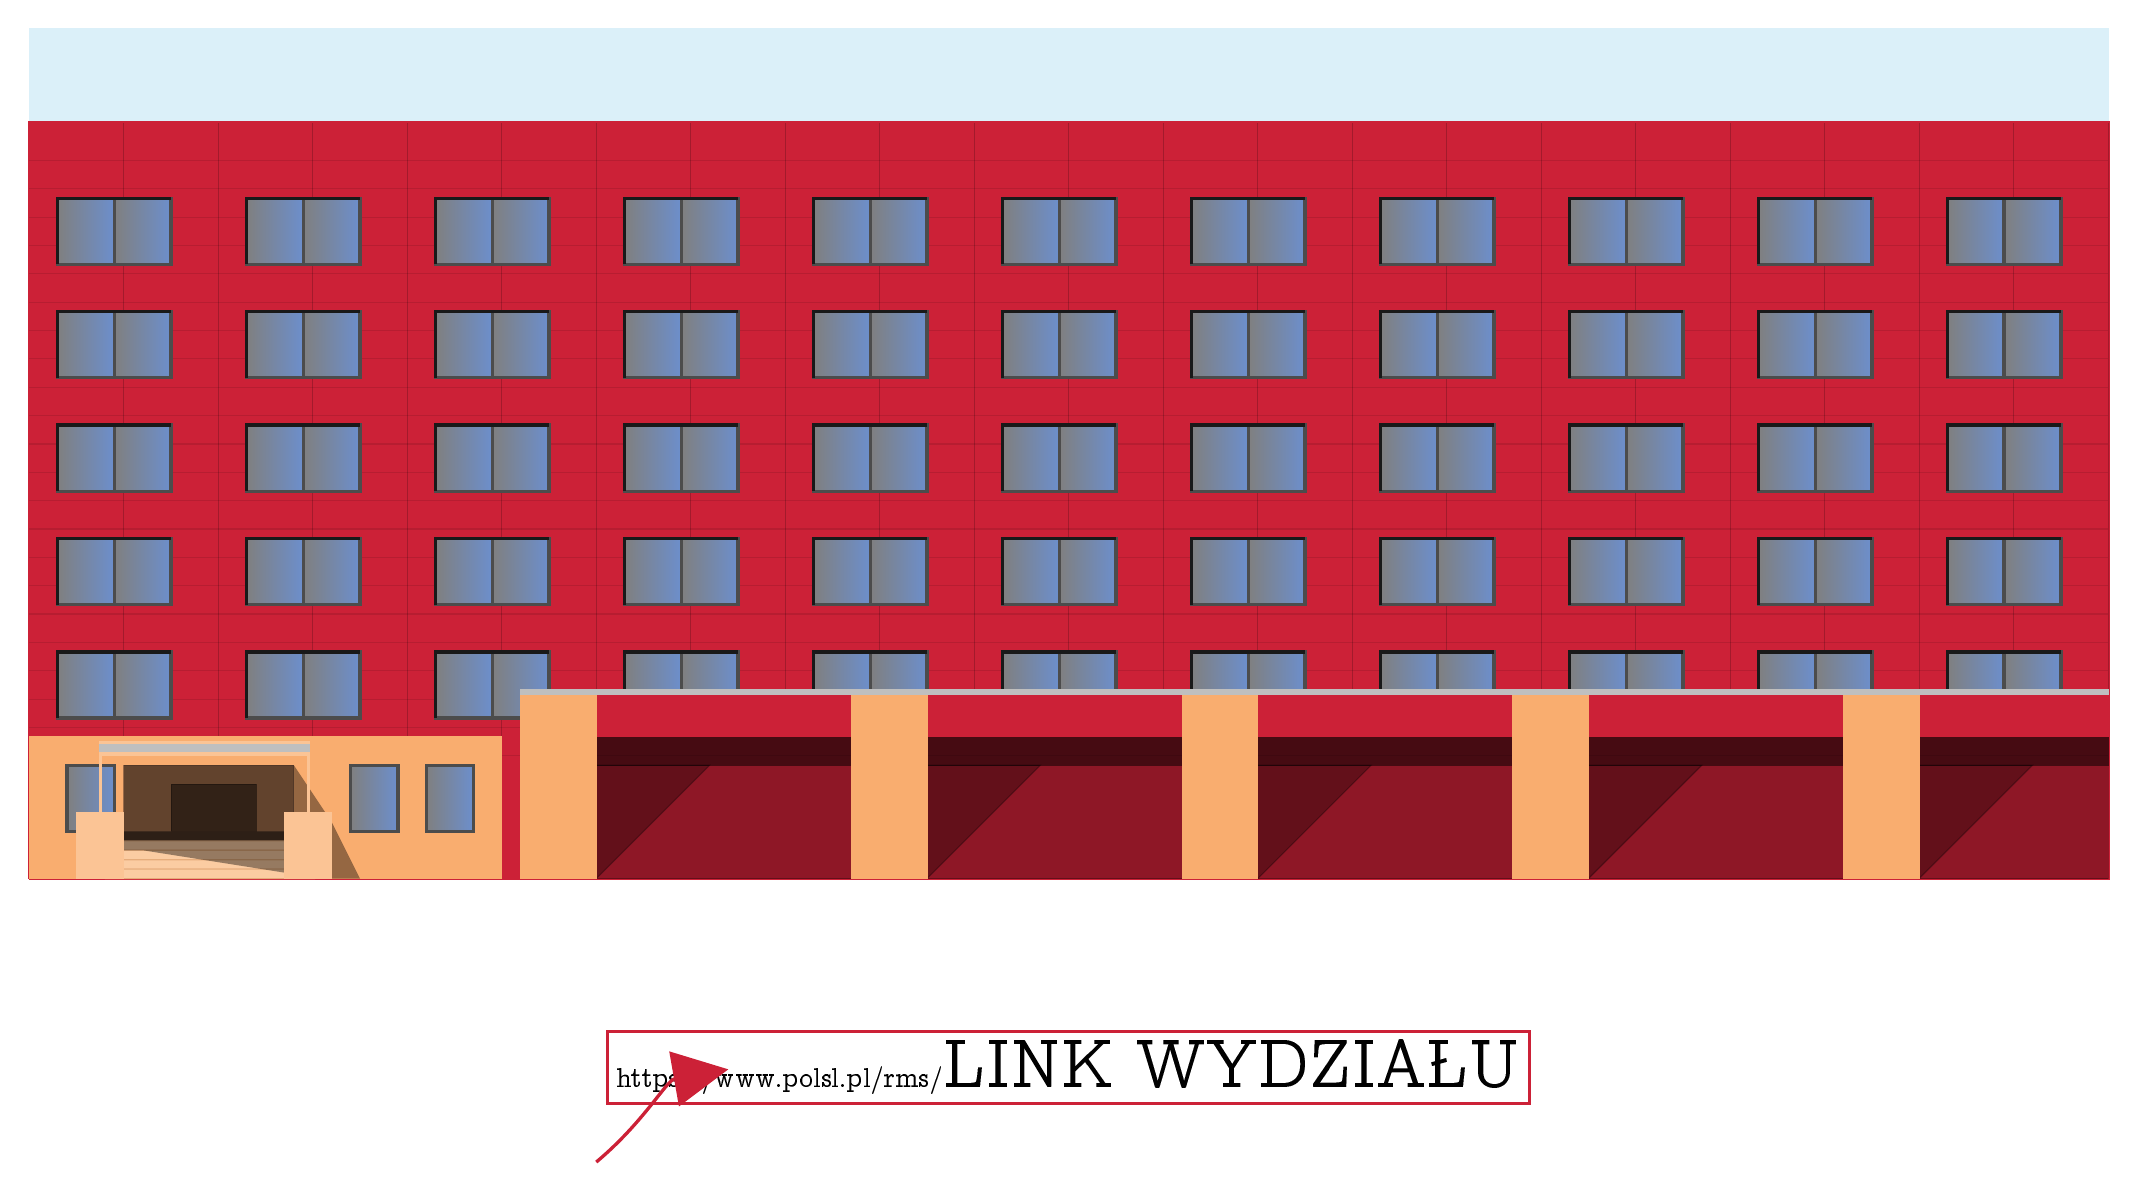
\begin{tikzpicture}[scale=1.2]
%\draw[help lines] (0,0) grid (21,10);
\filldraw[SkyBlue!30](0,1)rectangle(22,10);
\draw[BrickRed!60!WildStrawberry,fill=BrickRed!60!WildStrawberry,very thick] (0,1) to(0,9) to(22,9) to (22,1) to(0,1);

%%%% kratka %%%%
\foreach \j in {1,2,...,22}{
\draw[black,opacity=0.2](\j,2.5)to(\j,9);
\draw[black,opacity=0.1](0,0.3*\j+2)to(22,0.3*\j+2);
}

%%%% okna %%%%
\foreach \j in {2,3,...,6}{

\foreach \i in {0,...,10}{
\filldraw[Black!70,left color=gray, right color=gray!30!CornflowerBlue,very thick] (2*\i+0.3, 1.2*\j+0.3) rectangle (2*\i+0.9, 1.2*\j+1);
\filldraw[Black!70,left color=gray, right color=gray!30!CornflowerBlue,very thick] (2*\i+0.9, 1.2*\j+0.3) rectangle (2*\i+1.5, 1.2*\j+1);

\draw[Black!90,very thick](2*\i+0.3, 1.2*\j+0.3)to(2*\i+0.3, 1.2*\j+1)to(2*\i+1.5, 1.2*\j+1);
}
}

%%%% przód %%%%
\filldraw[Black,opacity=0.5](5.2,2.2)rectangle(22,3);
\filldraw[Black,opacity=0.3](5.2,1)rectangle(22,3);

\filldraw[BrickRed!60!WildStrawberry](5.2,2.5)rectangle(22,3);
\foreach \j in {2,3,...,6}{
\filldraw[Black,opacity=0.3](3.5*\j-1,1)to(3.5*\j+0.2,2.2)to(3.5*\j-1,2.2);}
\foreach \j in {2,3,...,6}{
\filldraw[Apricot](3.5*\j-1,1)rectangle(3.5*\j-1.8,3);
}
\filldraw[Gray!50](5.2,2.95)rectangle(22,3);

%%%% wejście %%%%

\filldraw[Apricot](0,1)rectangle(5,2.5);
\filldraw[Black!70,left color=gray, right color=gray!30!CornflowerBlue,very thick] (0.4,1.5) rectangle (0.9,2.2);
\filldraw[Black!70,left color=gray, right color=gray!30!CornflowerBlue,very thick] (4.2,1.5) rectangle (4.7,2.2);
\filldraw[Black!70,left color=gray, right color=gray!30!CornflowerBlue,very thick] (3.4,1.5) rectangle (3.9,2.2);

\filldraw[Black!50!Apricot,opacity=0.7](1,1.5)rectangle(2.8,2.2);
\filldraw[Black!80!Apricot,opacity=0.7](1.5,1.5)rectangle(2.4,2);
\filldraw[Black!70!Apricot,draw=none](1,1.5)to(2.8,1.5)to(2.9,1.4)to(0.9,1.4);
\filldraw[color=Apricot!80!Gray,fill=Apricot!60](1,1.4)to(2.8,1.4)to(2.9,1.3)to(0.9,1.3);
\filldraw[color=Apricot!80!Gray,fill=Apricot!60](1,1.3)to(2.8,1.3)to(2.9,1.2)to(0.9,1.2);
\filldraw[color=Apricot!80!Gray,fill=Apricot!60](1,1.2)to(2.8,1.2)to(2.95,1.1)to(0.85,1.1);
\filldraw[color=Apricot!80!Gray,fill=Apricot!60](1,1.1)to(2.8,1.1)to(3,1)to(0.8,1);
\filldraw[Black, opacity=0.4,draw=none](1,1.5)to(1,2.2)to(2.8,2.2)to(3.2,1.6)to(3.5,1)to(3.1,1)to(1.2,1.3)to(1,1.3);


%%%% filary %%%%
\filldraw[Apricot!70](0.5,1)rectangle(1,1.7);
\filldraw[Apricot!70](0.74,1)rectangle(0.76,2.4);
\filldraw[Apricot!70](2.7,1)rectangle(3.2,1.7);
\filldraw[Apricot!70](2.96,1)rectangle(2.94,2.4);
\filldraw[Apricot!70](0.74,2.3)rectangle(2.96,2.45);
\filldraw[Gray!50](0.74,2.35)rectangle(2.96,2.42);

%%%% odnośnik %%%%
\node [draw=BrickRed!60!WildStrawberry,very thick]at (11,-1) {\href{https://www.polsl.pl/rms/}{\Huge{LINK WYDZIAŁU}}};
\node[draw=none] (A) at(7.5,-1){};
\draw [-{Triangle[length=7mm, width=7mm]},very thick,draw=BrickRed!60!WildStrawberry] (6,-2) to [out=40,in=-170] (A);
\end{tikzpicture}

%%%%%%%%%%%%%%%%%%%%%%%%%%% RAU %%%%%%%%%%%%%%%%%%%%%%%%%%%%%%

\newpage
\centering\hypertarget{rau}{{\Huge{RAU}}}

\vspace{2cm}
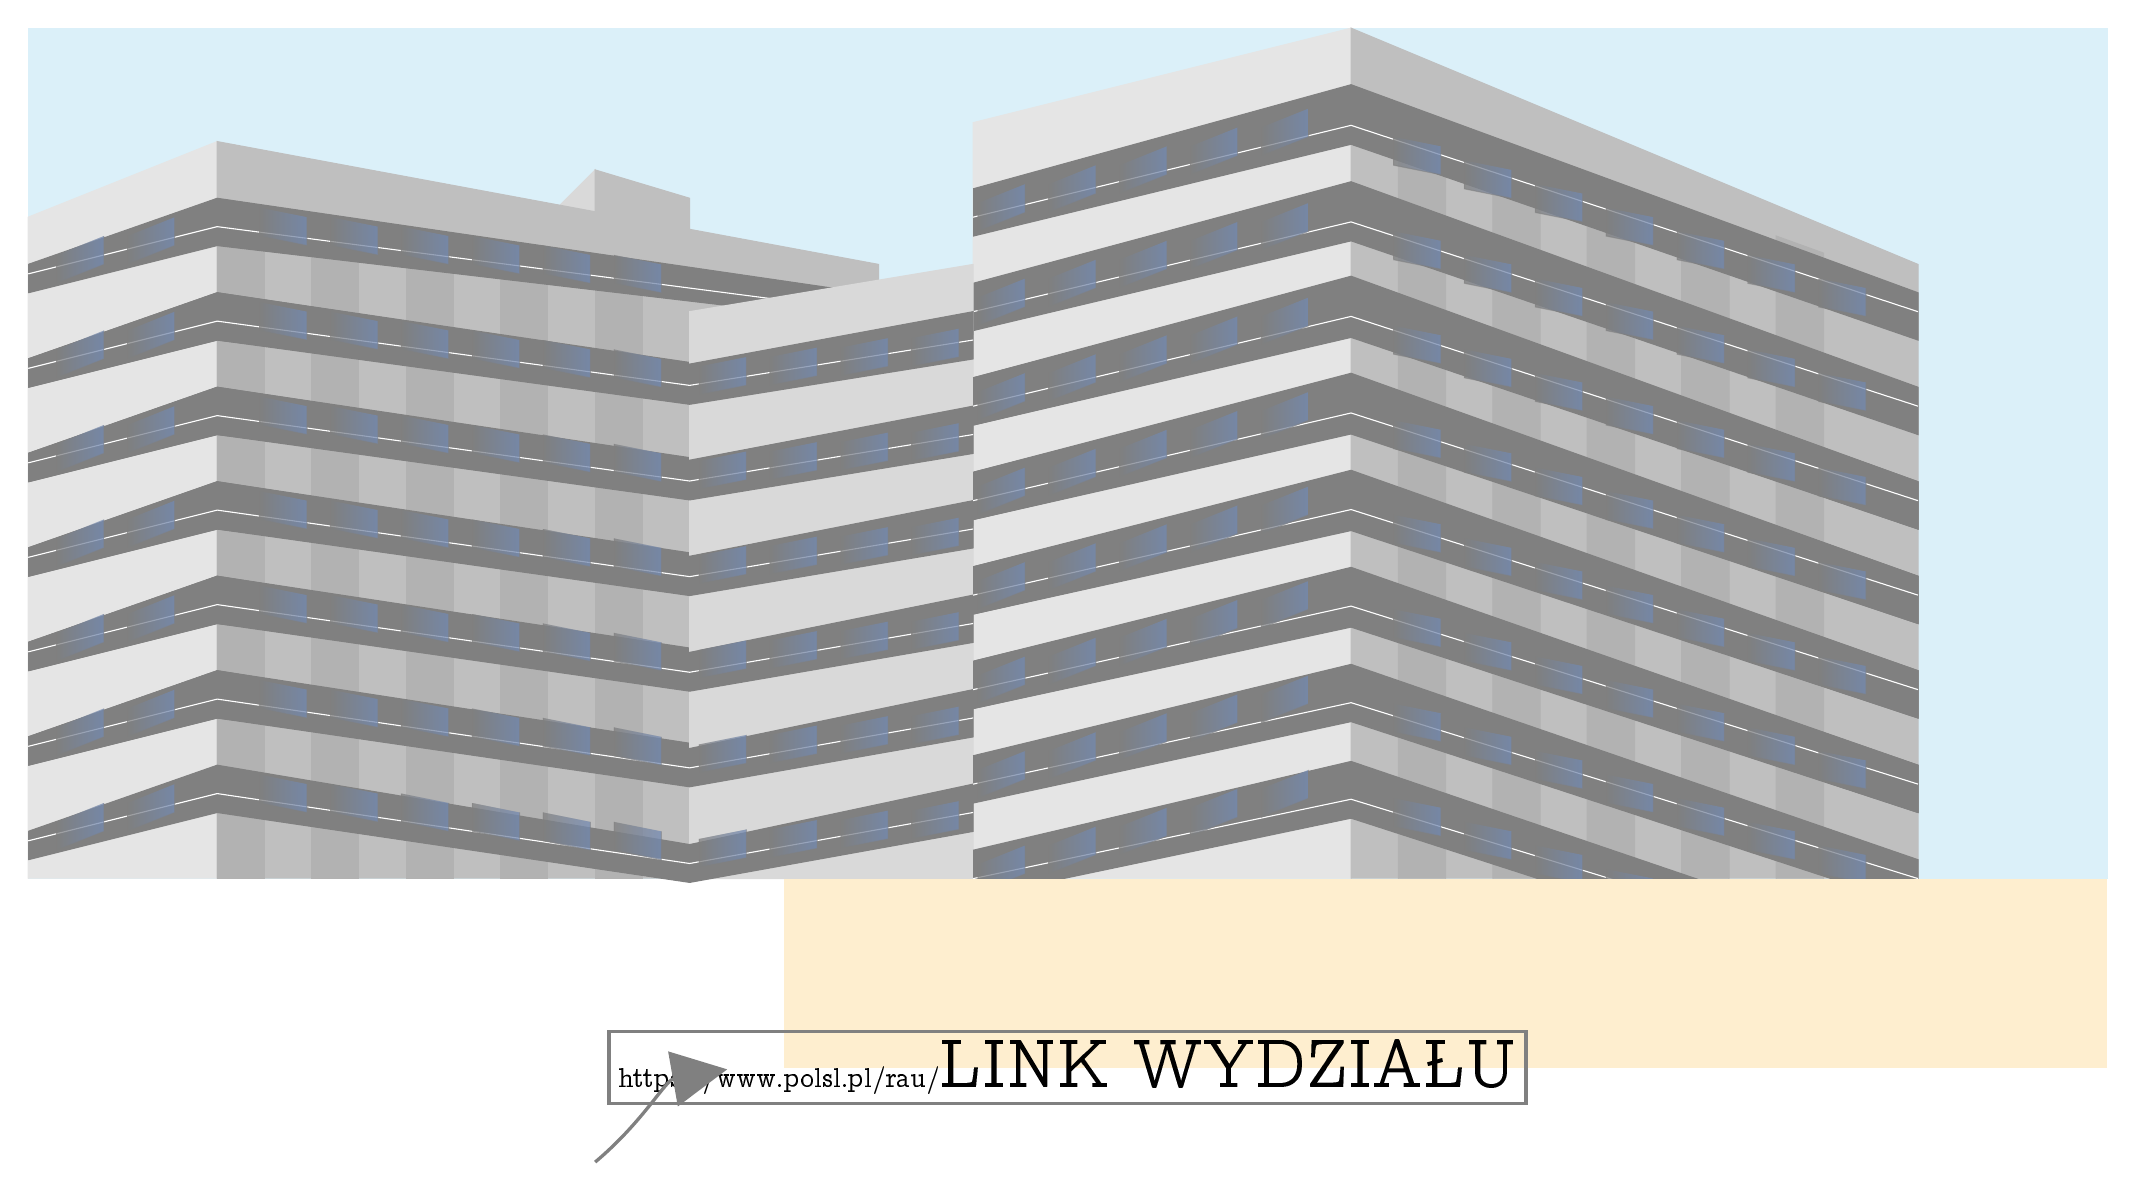
\begin{tikzpicture}[scale=1.2]
%\draw[help lines] (0,0) grid (21,10);
\filldraw[SkyBlue!30](0,1)rectangle(22,10);

%%%% ściany główne %%%%
\filldraw[Gray!20](0,1)to(0,8)to(2,8.8)to(2,1);
\filldraw[Gray!30](4.5,7)to(6,8.5)to(6,6);

\filldraw[Gray!50](2,1)to(2,8.8)to(9,7.5)to(9,1);
\filldraw[Gray!50](6,7.5)to(6,8.5)to(7,8.2)to(7,7);

\filldraw[Gray!20](10,1)to(10,9)to(14,10)to(14,1);
\filldraw[Gray!50](14,1)to(14,10)to(20,7.5)to(20,1);


%%%% paski I i  III %%%%

%% pion %%
\foreach \i in {2,...,6}{
\filldraw[Black!30](12.5+\i,1)to(12.5+\i,9-0.2*\i)to(12.5+\i+0.5,9-0.23*\i)to(12.5+\i+0.5,1);
\filldraw[Black!30](\i,1)to(\i,8-0.1*\i)to(\i+0.5,8-0.1*\i)to(\i+0.5,1);
}
%% poziom %%
\foreach \i in {1,...,6}{

\filldraw[Black!50](0,1.2+\i)to(2,1.7+\i)to(10,0.7\i+\i)to(10,1.2*0.8\i+\i)to(2,2.2+\i)to(0,1.5+\i);
\draw[white](0,1.4+\i)to(2,1.9+\i)to(10,0.7\i+0.1+\i);
\filldraw[Black!50](10,1.8+\i)to(14,2.2*1.2\i+\i)to(20,0.7+\i)to(20,1.2+\i)to(14,2.7*1.2\i+\i)to(10,2.3+\i);
\draw[white](10,2+\i)to(14,2.2*1.2\i+0.2+\i)to(20,0.9+0.1+\i);
}

\filldraw[Gray!30](7,1)to(7,7)to(10,7.5)to(10,1)to(7,1);

%%%% paski II %%%% 

%%poziom%%
\foreach \i in {0,1,2,...,5}{
\filldraw[Black!50](0,1.2+\i)to(2,1.7+\i)to(7,1.2*0.8\i+\i)to(10,1.5+\i)to(10,2+\i)to(7,1.7*0.8\i+\i)to(2,2.2+\i)to(0,1.5+\i);
\draw[white](0,1.4+\i)to(2,1.9+\i)to(7,1.2*0.8\i+0.2+\i)to(10,1.7+\i);

%% poprawa paski III %%
\filldraw[Black!50](10,1.8+\i-1)to(14,2.2*1.2\i+\i-1)to(20,0.7+\i-1)to(20,1.2+\i-1)to(14,2.7*1.2\i+\i-1)to(10,2.3+\i-1);
\draw[white](10,2+\i-1)to(14,2.2*1.2\i+0.2+\i-1)to(20,0.9+0.1+\i-1);
}

%%%% okna %%%%

\foreach \j in {1.6,2.1,2.6,3.1,3.6,4.1,4.6}{
\foreach \i in {1.5,2,2.5,...,4}{
\filldraw[gray,left color=gray, right color=gray!30!CornflowerBlue,opacity=0.5] (1.5*\i+0.2, 2*\j-1-0.2*\i+0.2) to (1.5*\i+0.2, 2*\j-1.3-0.2*\i+0.2)to (1.5*\i+0.7, 2*\j-1.4-0.2*\i+0.2) to(1.5*\i+0.7, 2*\j-1.1-0.2*\i+0.2);
}}

\foreach \j in {3.8,4.3,4.8,5.3,5.8,6.3,6.8,7.3}{
\foreach \i in {9.5,10,10.5,11,11.5,12,12.5}{
\filldraw[gray,left color=gray, right color=gray!30!CornflowerBlue,opacity=0.5] (1.5*\i+0.2, 2*\j-1-0.5*\i) to (1.5*\i+0.2, 2*\j-1.3-0.5*\i)to (1.5*\i+0.7, 2*\j-1.4-0.5*\i) to(1.5*\i+0.7, 2*\j-1.1-0.5*\i);
}}
\foreach \j in {0.8,1.3,1.8,2.3,2.8,3.3}{
\foreach \i in {4.6,5.1,5.6,6.1}{
\filldraw[gray,left color=gray, right color=gray!30!CornflowerBlue,opacity=0.5] (1.5*\i+0.2, 2*\j-1.1+0.2*\i) to (1.5*\i+0.2, 2*\j-1.4+0.2*\i)to (1.5*\i+0.7, 2*\j-1.3+0.2*\i) to(1.5*\i+0.7, 2*\j-1+0.2*\i);
}}

\foreach \j in {0.2,0.7,1.2,1.7,2.2,2.7,3.2,3.7}{
\foreach \i in {6.5,7,7.5,8,8.5}{
\filldraw[gray,left color=gray, right color=gray!30!CornflowerBlue,opacity=0.5] (1.5*\i+0.3, 2*\j-1.2+0.4*\i-0.65) to (1.5*\i+0.3, 2*\j-1.5+0.4*\i-0.65)to (1.5*\i+0.8, 2*\j-1.3+0.4*\i-0.65) to(1.5*\i+0.8, 2*\j-1+0.4*\i-0.65);
}}

\foreach \j in {0.7,1.2,1.7,2.2,2.7,3.2,3.7}{
\foreach \i in {0,0.5}{
\filldraw[gray,left color=gray, right color=gray!30!CornflowerBlue,opacity=0.5] (1.5*\i+0.3, 2*\j-1.2+0.4*\i+1.4) to (1.5*\i+0.3, 2*\j-1.5+0.4*\i+1.4)to (1.5*\i+0.8, 2*\j-1.3+0.4*\i+1.4) to(1.5*\i+0.8, 2*\j-1+0.4*\i+1.4);
}}

\filldraw[Dandelion!20,draw=none](8,-1)rectangle(22,1);
%%%% odnośnik %%%%
\node [draw=Black!50,very thick] at (11,-1) {\href{https://www.polsl.pl/rau/}{\Huge{LINK WYDZIAŁU}}};
\node[draw=none] (A) at(7.5,-1){};
\draw [-{Triangle[length=7mm, width=7mm]},very thick,draw=Black!50] (6,-2) to [out=40,in=-170] (A);
\end{tikzpicture}

%%%%%%%%%%%%%%%%%%%%%%%%%%% RG %%%%%%%%%%%%%%%%%%%%%%%%%%%%%%

\newpage
\centering\hypertarget{rg}{{\Huge{RG}}}

\vspace{2cm}
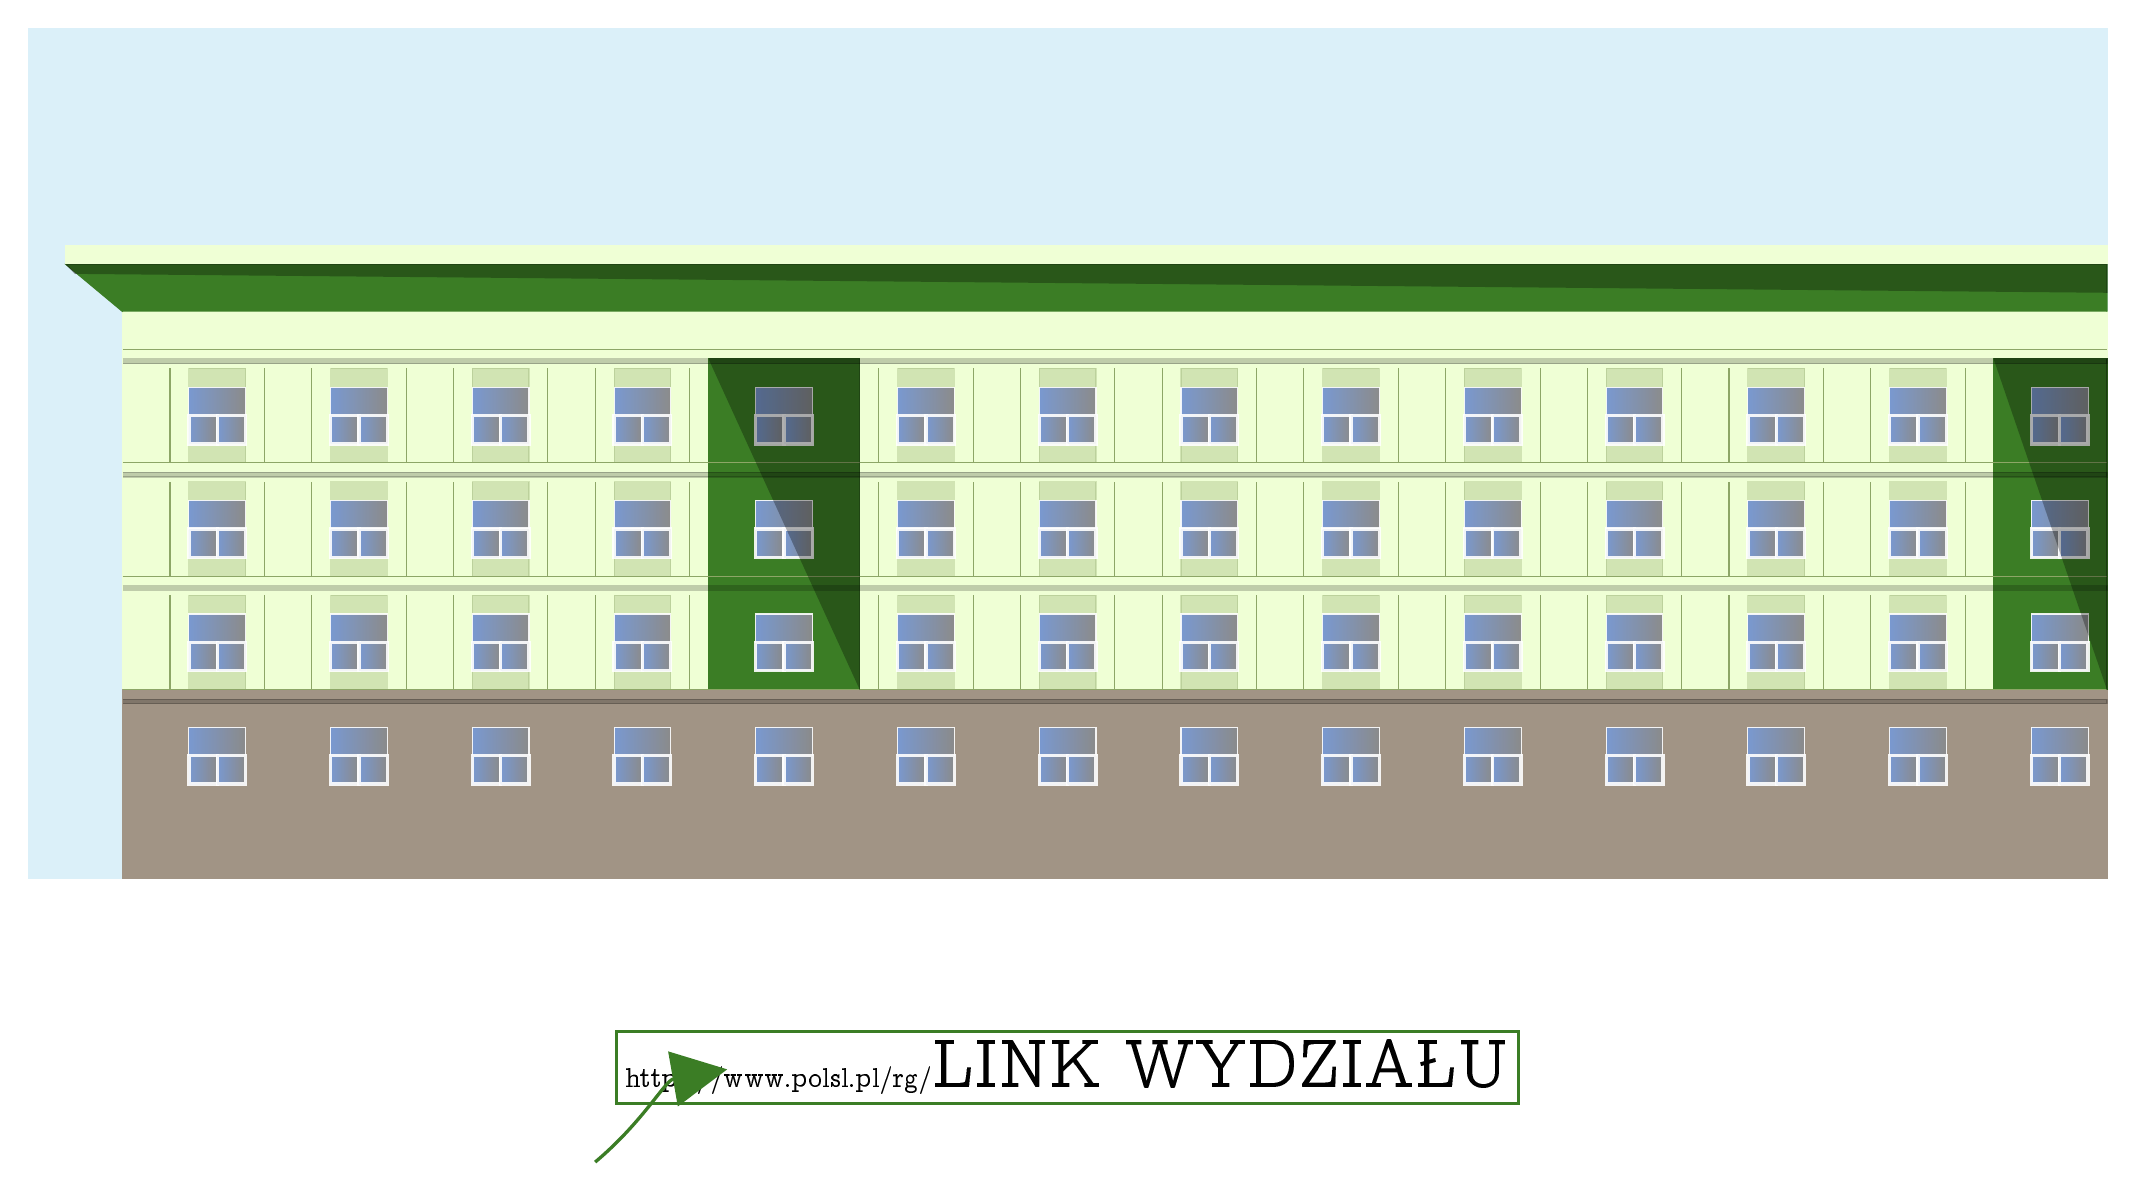
\begin{tikzpicture}[scale=1.2]
%\draw[help lines] (0,0) grid (21,10);
\filldraw[SkyBlue!30](0,1)rectangle(22,10);

\filldraw[GreenYellow!20](1,1)to(1,7)to(22,7)to(22,1);

%%%% dach %%%%
\filldraw[OliveGreen](1,7)to(0.4,7.5)to(22,7.5)to(22,7);
\filldraw[Black,opacity=0.3](0.5,7.4)to(0.4,7.5)to(22,7.5)to(22,7.2);
\filldraw[GreenYellow!20](0.4,7.5)to(0.4,7.7)to(22,7.7)to(22,7.5);

%%%% fundamenty %%%%
\filldraw[Tan!40!Gray](1,1)to(1,3)to(22,3)to(22,1);

%%%% zielone wnęki %%%%
\filldraw[OliveGreen](7.2,3)to(7.2,6.5)to(8.8,6.5)to(8.8,3);
\filldraw[OliveGreen](20.8,3)to(20.8,6.5)to(22,6.5)to(22,3);

%%%% paski %%%%
\foreach \j in {0,1.2,2.4}{
\foreach \i in {1,2,3,4,6,7,8,9,10,...,13}{
\draw[GreenYellow!30!Gray](\i*1.5,3+\j)to(\i*1.5,4+\j);
\draw[GreenYellow!30!Gray](\i*1.5+1,3+\j)to(\i*1.5+1,4+\j);
\filldraw[GreenYellow!30!Gray,opacity=0.3](\i*1.5+0.2,3+\j)to(\i*1.5+0.2,4+\j)to(\i*1.5-0.2+1,4+\j)to(\i*1.5-0.2+1,3+\j);
}}

%%%% okna %%%%
\foreach \j in {1,2,3,4}{
\foreach \i in {1.5,3,...,21}{
\filldraw[white,left color=gray!30!CornflowerBlue, right color=gray,opacity=0.9] (\i+0.2, 1.2*\j+1.1) rectangle (\i+0.8, 1.2*\j+1.4);
\filldraw[White,left color=gray!30!CornflowerBlue, right color=gray,very thick,opacity=0.9] (\i+0.2, 1.2*\j+0.8) rectangle (\i+0.5, 1.2*\j+1.1);
\filldraw[White,left color=gray!30!CornflowerBlue, right color=gray,very thick,opacity=0.9] (\i+0.5, 1.2*\j+0.8) rectangle (\i+0.8, 1.2*\j+1.1);
}

%%%% wnęki okienne %%%%
\draw[GreenYellow!30!Gray](1, 1.2*\j+1.8)to(22, 1.2*\j+1.8);
\filldraw[Black,opacity=0.2](1, 1.2*\j+1.7)to(22, 1.2*\j+1.7)to(22, 1.2*\j+1.65)to(1, 1.2*\j+1.65);
}

%%%% cienie %%%%
\filldraw[Black,opacity=0.3](7.2,6.5)to(8.8,6.5)to(8.8,3);
\filldraw[Black,opacity=0.3](20.8,6.5)to(22,6.5)to(22,3);

%%%% odnośnik %%%%
\node [draw=OliveGreen,very thick] at (11,-1) {\href{https://www.polsl.pl/rg/}{\Huge{LINK WYDZIAŁU}}};
\node[draw=none] (A) at(7.5,-1){};
\draw [-{Triangle[length=7mm, width=7mm]},very thick,draw=OliveGreen] (6,-2) to [out=40,in=-170] (A);
\end{tikzpicture}

%%%%%%%%%%%%%%%%%%%%%%%%%%% RCh %%%%%%%%%%%%%%%%%%%%%%%%%%%%%%

\newpage
\centering\hypertarget{rch}{{\Huge{RCh}}}

\vspace{2cm}
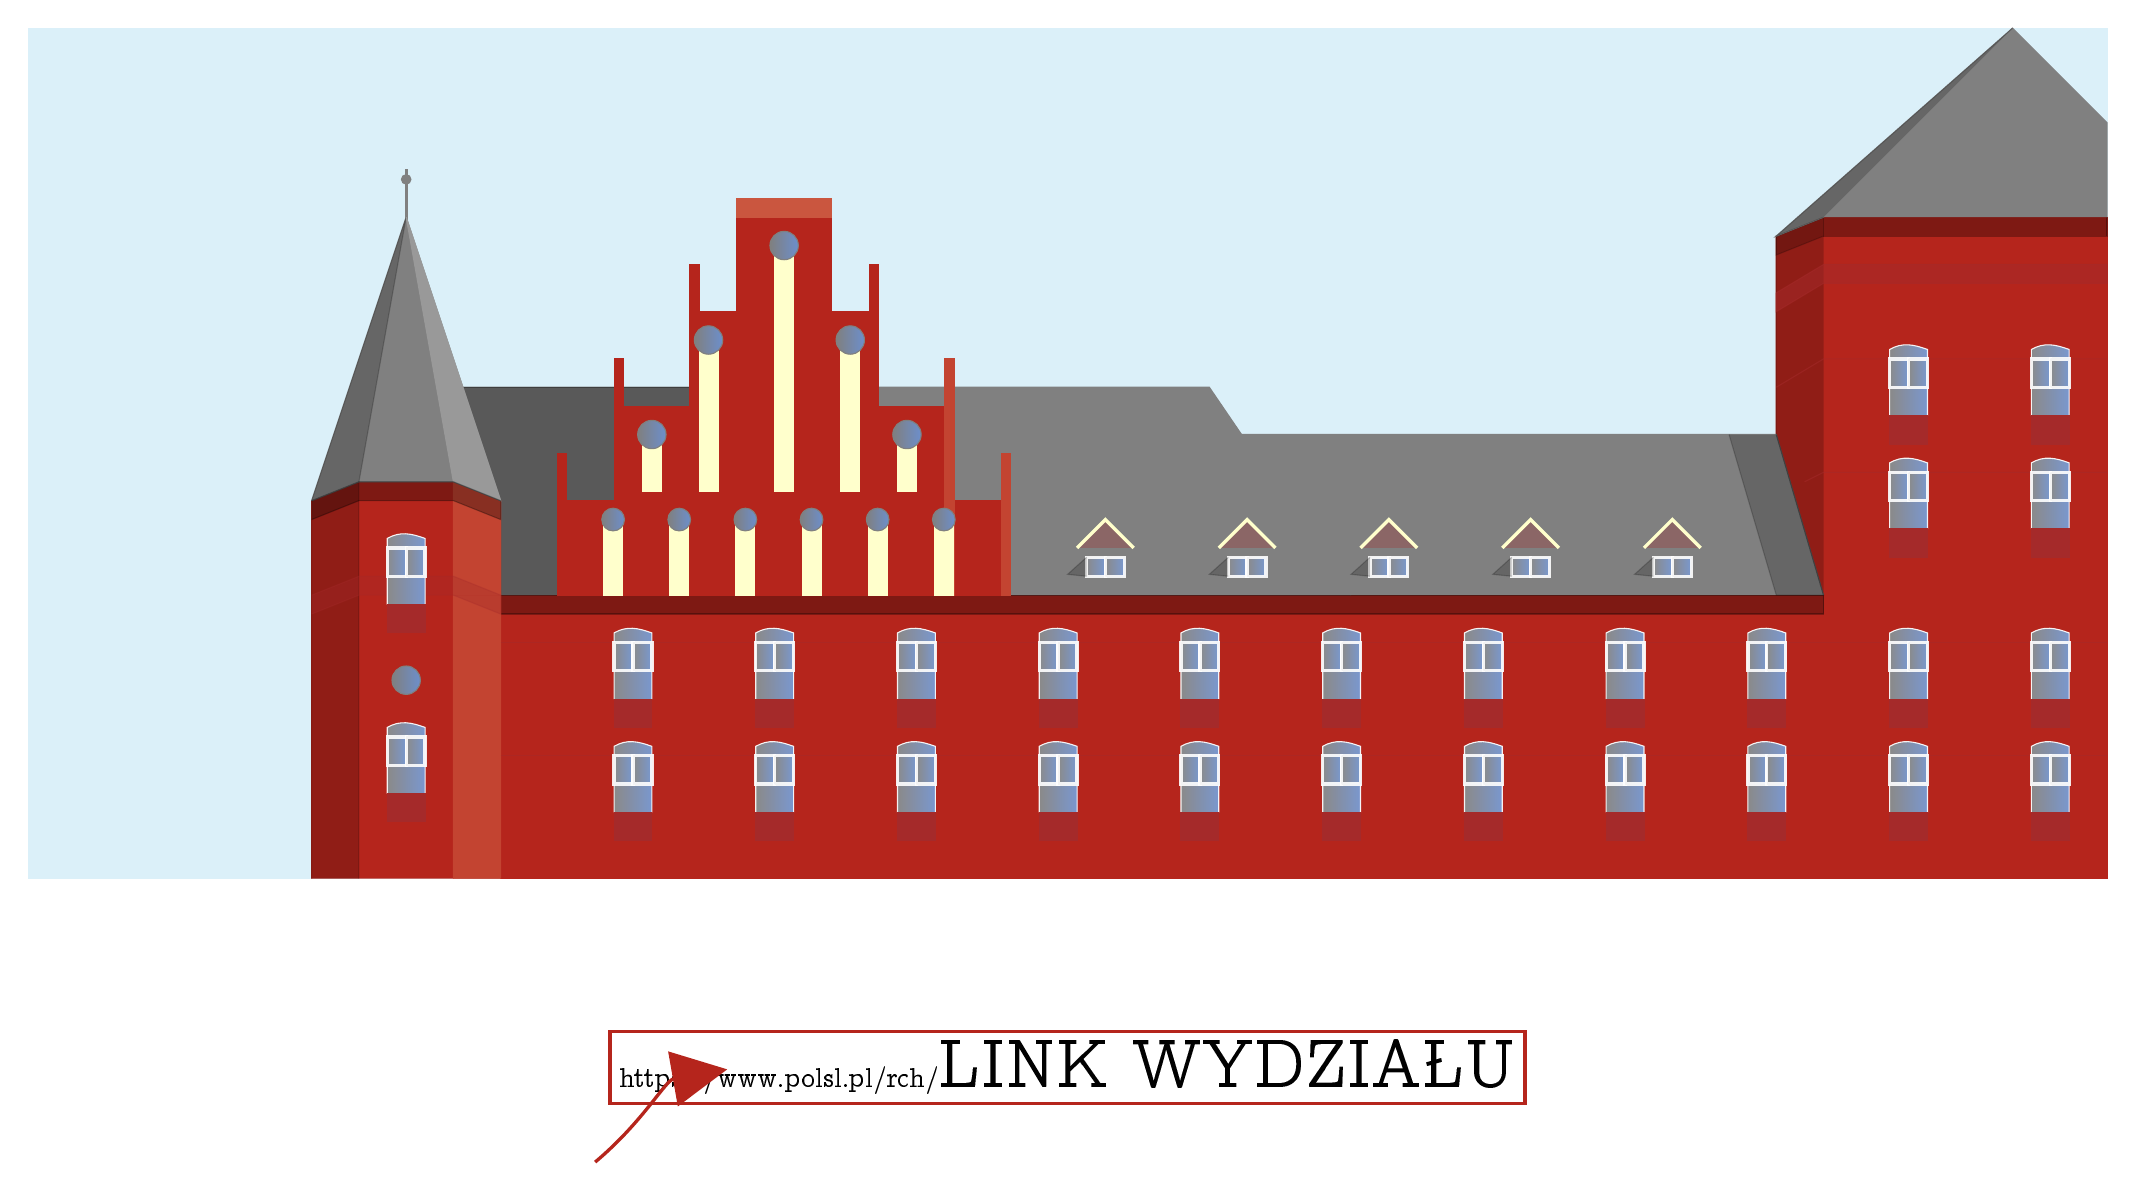
\begin{tikzpicture}[scale=1.2]
%\draw[help lines] (0,0) grid (21,10);
\filldraw[SkyBlue!30](0,1)rectangle(22,10);

\filldraw[BrickRed](5,1)rectangle(22,4);
\filldraw[BrickRed](19,8)to(18.5,7.8)to(18.5,4)to(19,4);

\filldraw[BrickRed](19,1)rectangle(22,8);
\filldraw[BrickRed](7.5,4)rectangle(8.5,8);
\filldraw[BrickRed!70](7.5,8)rectangle(8.5,8.2);

%%%% dach paski i cienie %%%%

\filldraw[gray](7,4)to(7,5.7)to(18.5,5.7)to(19,4);
\filldraw[gray](4,4)to(4,6.2)to(12.5,6.2)to(14,4);
\filldraw[Black,opacity=0.3](4,4)to(4,6.2)to(8,6.2)to(8,4);
\filldraw[Black,opacity=0.3](5,4)to(19,4)to(19,3.8)to(5,3.8);
\filldraw[Black,opacity=0.3](19,8)to(19,7.8)to(22,7.8)to(22,8);
\filldraw[Black,opacity=0.2](19,8)to(18.5,7.8)to(18.5,5.7)to(19,4);
\filldraw[Black,opacity=0.2](19,8)to(18.5,7.8)to(18.5,7.6)to(19,7.8);
\filldraw[Black,opacity=0.2](18.5,5.7)to(19,4)to(18.5,4)to(18,5.7);
\filldraw[gray](19,8)to(21,10)to(22,9)to(22,8);
\filldraw[gray](19,8)to(18.5,7.8)to(21,10);
\filldraw[Black,opacity=0.2](19,8)to(18.5,7.8)to(21,10);

\filldraw[BrickRed](5.6,4)rectangle(10.4,5);
\filldraw[BrickRed](5.6,4)rectangle(5.7,5.5);
\filldraw[BrickRed!80](10.3,4)rectangle(10.4,5.5);
\filldraw[BrickRed](6.2,4)rectangle(9.8,6);
\filldraw[BrickRed](6.2,4)rectangle(6.3,6.5);
\filldraw[BrickRed!80](9.7,4)rectangle(9.8,6.5);
\filldraw[BrickRed](7,4)rectangle(9,7);
\filldraw[BrickRed](7,4)rectangle(7.1,7.5);
\filldraw[BrickRed](8.9,4)rectangle(9,7.5);

\filldraw[BrickRed](3,1)to(3,4)to(3.5,4.2)to(4.5,4.2)to(5,4)to(5,1);

\filldraw[BrickRed!80](4.5,1)to(4.5,4.2)to(5,4)to(5,1);
\filldraw[BrickRed](3,4)to(3,5)to(3.5,5.2)to(4.5,5.2)to(5,5)to(5,4);
\filldraw[BrickRed!80](4.5,4)to(4.5,5.2)to(5,5)to(5,4);
\filldraw[Black,opacity=0.2](3,1)to(3,5)to(3.5,5.2)to(3.5,1);

\filldraw[gray](3,5)to(3.5,5.2)to(4.5,5.2)to(5,5)to(4,8)to(3,5);
\filldraw[gray](3.99,7.9)rectangle(4.01,8.5);
\filldraw[gray](4,8.4)circle(0.05);
\filldraw[Black,opacity=0.2](3,5)to(4,8)to(3.5,5.2);
\filldraw[gray!80](4.5,5.2)to(4,8)to(5,5);
\draw[Brown,opacity=0.5](5,3.5)to(22,3.5);
\draw[Brown,opacity=0.5](5,2.3)to(22,2.3);
\draw[Brown,opacity=0.5](18.8,5.2)to(19,5.3)to(22,5.3);
\draw[Brown,opacity=0.5](18.5,6.2)to(19,6.5)to(22,6.5);
\filldraw[Brown,opacity=0.5](18.5,7.2)to(19,7.5)to(22,7.5)to(22,7.3)to(19,7.3)to(18.5,7)to(18.5,7.2);
\filldraw[Black, opacity=0.3](3,5)to(3.5,5.2)to(4.5,5.2)to(5,5)to(5,4.8)to(4.5,5)to(3.5,5)to(3,4.8);
\filldraw[Brown, opacity=0.3](3,4)to(3.5,4.2)to(4.5,4.2)to(5,4)to(5,3.8)to(4.5,4)to(3.5,4)to(3,3.8);

%%%% okna wieża %%%%

\filldraw[white,left color=gray, right color=gray!30!CornflowerBlue,opacity=0.9] (3.8, 3.9) to(3.8, 4.6) to[out=30,in=-200](4.2, 4.6) to(4.2,3.9);
\filldraw[White,left color=gray, right color=gray!30!CornflowerBlue,very thick,opacity=0.9] (3.8,4.2) rectangle (4, 4.5);
\filldraw[White,left color=gray, right color=gray!30!CornflowerBlue,very thick,opacity=0.9] (4,4.2) rectangle (4.2, 4.5);
\filldraw[Brown](3.8, 3.6) rectangle (4.2, 3.9);

\filldraw[Gray,left color=gray, right color=gray!30!CornflowerBlue](4,3.1)circle(0.15);

\filldraw[white,left color=gray, right color=gray!30!CornflowerBlue,opacity=0.9] (3.8, 1.9) to(3.8, 2.6) to[out=30,in=-200](4.2, 2.6) to(4.2,1.9);
\filldraw[White,left color=gray, right color=gray!30!CornflowerBlue,very thick,opacity=0.9] (3.8,2.2) rectangle (4, 2.5);
\filldraw[White,left color=gray, right color=gray!30!CornflowerBlue,very thick,opacity=0.9] (4,2.2) rectangle (4.2, 2.5);
\filldraw[Brown](3.8, 1.6) rectangle (4.2, 1.9);


%%%% okna okrągłe %%%%
\foreach \i in {8.7,9.7,...,13.7}{
\filldraw[Yellow!20](\i-0.3*\i,4)rectangle(\i+0.2-0.3*\i,4.8);
\filldraw[Gray,left color=gray, right color=gray!30!CornflowerBlue](\i+0.1-0.3*\i,4.8)circle(0.12);
}

\filldraw[Yellow!20](6.5,5.1)rectangle(6.7,5.7);
\filldraw[Gray,left color=gray, right color=gray!30!CornflowerBlue](6.6,5.7)circle(0.15);
\filldraw[Yellow!20](7.1,5.1)rectangle(7.3,6.7);
\filldraw[Gray,left color=gray, right color=gray!30!CornflowerBlue](7.2,6.7)circle(0.15);
\filldraw[Yellow!20](7.9,5.1)rectangle(8.1,7.7);
\filldraw[Gray,left color=gray, right color=gray!30!CornflowerBlue](8,7.7)circle(0.15);
\filldraw[Yellow!20](8.6,5.1)rectangle(8.8,6.7);
\filldraw[Gray,left color=gray, right color=gray!30!CornflowerBlue](8.7,6.7)circle(0.15);
\filldraw[Yellow!20](9.2,5.1)rectangle(9.4,5.7);
\filldraw[Gray,left color=gray, right color=gray!30!CornflowerBlue](9.3,5.7)circle(0.15);


%%%% okna główne %%%%

\foreach \j in {1,2}{
\foreach \i in {6,7.5,...,21}{
\filldraw[white,left color=gray, right color=gray!30!CornflowerBlue,opacity=0.9] (\i+0.2, 1.2*\j+0.5) to(\i+0.2, 1.2*\j+1.2) to[out=30,in=-200](\i+0.6, 1.2*\j+1.2) to(\i+0.6, 1.2*\j+0.5);
\filldraw[White,left color=gray, right color=gray!30!CornflowerBlue,very thick,opacity=0.9] (\i+0.2, 1.2*\j+0.8) rectangle (\i+0.4, 1.2*\j+1.1);
\filldraw[White,left color=gray, right color=gray!30!CornflowerBlue,very thick,opacity=0.9] (\i+0.4, 1.2*\j+0.8) rectangle (\i+0.6, 1.2*\j+1.1);
\filldraw[Brown](\i+0.2, 1.2*\j+0.5) rectangle (\i+0.6, 1.2*\j+0.2);
}}


%%%% okna dach %%%% 
\foreach \i in {11,12.5,...,17}{

\filldraw[White,left color=gray, right color=gray!30!CornflowerBlue,very thick,opacity=0.9] (\i+0.2, 4.2) rectangle (\i+0.4, 4.4);
\filldraw[White,left color=gray, right color=gray!30!CornflowerBlue,very thick,opacity=0.9] (\i+0.4, 4.2) rectangle (\i+0.6, 4.4);
\filldraw[Black,opacity=0.2](\i+0.2,4.2)to(\i,4.22)to(\i+0.2,4.4);
\filldraw[Brown,opacity=0.3](\i+0.1,4.5)to(\i+0.4,4.8)to(\i+0.7,4.5);
\draw[Yellow!20,very thick](\i+0.1,4.5)to(\i+0.4,4.8)to(\i+0.7,4.5);
}

%%%% okna prawo %%%%

\foreach \j in {3.5,4.5}{
\foreach \i in {19.5,21}{
\filldraw[white,left color=gray, right color=gray!30!CornflowerBlue,opacity=0.9] (\i+0.2, 1.2*\j+0.5) to(\i+0.2, 1.2*\j+1.2) to[out=30,in=-200](\i+0.6, 1.2*\j+1.2) to(\i+0.6, 1.2*\j+0.5);
\filldraw[White,left color=gray, right color=gray!30!CornflowerBlue,very thick,opacity=0.9] (\i+0.2, 1.2*\j+0.8) rectangle (\i+0.4, 1.2*\j+1.1);
\filldraw[White,left color=gray, right color=gray!30!CornflowerBlue,very thick,opacity=0.9] (\i+0.4, 1.2*\j+0.8) rectangle (\i+0.6, 1.2*\j+1.1);
\filldraw[Brown](\i+0.2, 1.2*\j+0.5) rectangle (\i+0.6, 1.2*\j+0.2);
}}

%%%% odnośnik %%%%
\node [draw=BrickRed,very thick]at (11,-1) {\href{https://www.polsl.pl/rch/}{\Huge{LINK WYDZIAŁU}}};
\node[draw=none] (A) at(7.5,-1){};
\draw [-{Triangle[length=7mm, width=7mm]},very thick,draw=BrickRed] (6,-2) to [out=40,in=-170] (A);
\end{tikzpicture}


\end{document}
